\documentclass[11pt,]{article}
\usepackage{lmodern}
\usepackage{amssymb,amsmath}
\usepackage{ifxetex,ifluatex}
\usepackage{fixltx2e} % provides \textsubscript
\ifnum 0\ifxetex 1\fi\ifluatex 1\fi=0 % if pdftex
  \usepackage[T1]{fontenc}
  \usepackage[utf8]{inputenc}
\else % if luatex or xelatex
  \ifxetex
    \usepackage{mathspec}
  \else
    \usepackage{fontspec}
  \fi
  \defaultfontfeatures{Ligatures=TeX,Scale=MatchLowercase}
\fi
% use upquote if available, for straight quotes in verbatim environments
\IfFileExists{upquote.sty}{\usepackage{upquote}}{}
% use microtype if available
\IfFileExists{microtype.sty}{%
\usepackage{microtype}
\UseMicrotypeSet[protrusion]{basicmath} % disable protrusion for tt fonts
}{}
\usepackage[margin=1.0in]{geometry}
\usepackage{hyperref}
\hypersetup{unicode=true,
            pdftitle={Evaluation of machine learning methods for 16S rRNA gene data},
            pdfborder={0 0 0},
            breaklinks=true}
\urlstyle{same}  % don't use monospace font for urls
\usepackage{graphicx,grffile}
\makeatletter
\def\maxwidth{\ifdim\Gin@nat@width>\linewidth\linewidth\else\Gin@nat@width\fi}
\def\maxheight{\ifdim\Gin@nat@height>\textheight\textheight\else\Gin@nat@height\fi}
\makeatother
% Scale images if necessary, so that they will not overflow the page
% margins by default, and it is still possible to overwrite the defaults
% using explicit options in \includegraphics[width, height, ...]{}
\setkeys{Gin}{width=\maxwidth,height=\maxheight,keepaspectratio}
\IfFileExists{parskip.sty}{%
\usepackage{parskip}
}{% else
\setlength{\parindent}{0pt}
\setlength{\parskip}{6pt plus 2pt minus 1pt}
}
\setlength{\emergencystretch}{3em}  % prevent overfull lines
\providecommand{\tightlist}{%
  \setlength{\itemsep}{0pt}\setlength{\parskip}{0pt}}
\setcounter{secnumdepth}{0}
% Redefines (sub)paragraphs to behave more like sections
\ifx\paragraph\undefined\else
\let\oldparagraph\paragraph
\renewcommand{\paragraph}[1]{\oldparagraph{#1}\mbox{}}
\fi
\ifx\subparagraph\undefined\else
\let\oldsubparagraph\subparagraph
\renewcommand{\subparagraph}[1]{\oldsubparagraph{#1}\mbox{}}
\fi

%%% Use protect on footnotes to avoid problems with footnotes in titles
\let\rmarkdownfootnote\footnote%
\def\footnote{\protect\rmarkdownfootnote}

%%% Change title format to be more compact
\usepackage{titling}

% Create subtitle command for use in maketitle
\newcommand{\subtitle}[1]{
  \posttitle{
    \begin{center}\large#1\end{center}
    }
}

\setlength{\droptitle}{-2em}

  \title{\textbf{Evaluation of machine learning methods for 16S rRNA gene data}}
    \pretitle{\vspace{\droptitle}\centering\huge}
  \posttitle{\par}
    \author{}
    \preauthor{}\postauthor{}
    \date{}
    \predate{}\postdate{}
  
\usepackage{booktabs}
\usepackage{longtable}
\usepackage{array}
\usepackage{multirow}
\usepackage[table]{xcolor}
\usepackage{wrapfig}
\usepackage{float}
\usepackage{colortbl}
\usepackage{pdflscape}
\usepackage{tabu}
\usepackage{threeparttable}
\usepackage{threeparttablex}
\usepackage[normalem]{ulem}
\usepackage{makecell}
\usepackage{caption}

\usepackage{helvet} % Helvetica font
\renewcommand*\familydefault{\sfdefault} % Use the sans serif version of the font
\usepackage[T1]{fontenc}

\usepackage[none]{hyphenat}

\usepackage{setspace}
\doublespacing
\setlength{\parskip}{1em}

\usepackage{lineno}

\usepackage{pdfpages}
\floatplacement{figure}{H} % Keep the figure up top of the page

\begin{document}
\maketitle

\vspace{35mm}

Running title: Machine learning methods in microbiome studies

\vspace{35mm}

Begüm D. Topçuoğlu\({^1}\), Nick Lesniak\({^1}\), Jenna Wiens\({^2}\),
Mack Ruffin\({^3}\), Patrick D. Schloss\textsuperscript{1\(\dagger\)}

\vspace{40mm}

\(\dagger\) To whom correspondence should be addressed:
\href{mailto:pschloss@umich.edu}{\nolinkurl{pschloss@umich.edu}}

1. Department of Microbiology and Immunology, University of Michigan,
Ann Arbor, MI 48109

2. Department of Computer Science and Engineering, University or
Michigan, Ann Arbor, MI 49109

3. Department of Family Medicine and Community Medicine, Penn State
Hershey Medical Center, Hershey, PA

\newpage

\linenumbers

\subsection{Abstract}\label{abstract}

Machine learning (ML) modeling of the human microbiome has the potential
to identify the microbial biomarkers and aid in diagnosis of many
chronic diseases such as inflammatory bowel disease, diabetes and
colorectal cancer. Progress has been made towards developing ML models
that predict health outcomes from bacterial abundances, but rigourous ML
models are scarce due to the flawed methods that call the validity of
developed ML models into question. Furthermore, the use of black box ML
models has hindered the validation of microbial biomarkers. To overcome
these challenges, we benchmarked seven different ML models that use
fecal 16S rRNA sequences to predict the presence/absence of colorectal
cancer (CRC) lesions (n=490 patients, 261 controls and 229 cases). To
show the effect of model selection, we assessed the predictive
performance, interpretability, and computational efficiency of the
following models: L2-regularized logistic regression, L1 and L2 support
vector machines (SVM) with linear and radial basis function kernels, a
decision tree, random forest, and extreme gradient boosting (XGBoost).
The random forest model was best at detecting CRC lesions with an AUROC
of 0.695 but it was slow to train (83.2 h) and hard to interpret.
Despite its simplicity, L2-regularized logistic regression followed
random forest in predictive performance with an AUROC of 0.680, and it
trained much faster (12 min). In this study, we showed that ML models
should be chosen based on expectations of predictive performance,
interpretability and available computational resources. Additionally, we
established standards for the development of modeling pipelines for
microbiome-associated ML models

\newpage

\subsection{Importance}\label{importance}

Prediction of health outcomes using ML is rapidly being adopted by
human-associated microbiome studies. However, the developed ML models so
far are overoptimistic in terms of validity and predictive performance.
Without rigorous ML pipelines, we cannot trust ML models. Before we can
speed up progress, we need to slow down, define and start using good ML
practices. \newpage

\subsection{Background}\label{background}

Advances in sequencing technology and decreasing costs of generating 16S
rRNA gene sequences have allowed rapid exploration of human associated
microbiome and its health implications. Currently, the human microbiome
field is growing at an unprecedented rate and as a result, there is an
increasing demand for methods that identify associations between members
of the microbiome and human health. However, this is difficult as human
associated microbial communities are remarkably complex,
high-dimensional and uneven within and between individuals with the same
disease. It is unlikely that a single species can explain a disease.
Instead, subsets of those communities, in relation to one another and to
their host, account for differences in health outcomes.

Machine learning (ML) methods are effective at recognizing and
highlighting patterns in complex microbial datasets. They learn from
existing data to predict the outcomes of new data and allow us to infer
on the reasons underlying that prediction. Therefore, researchers have
started to explore the utility of ML models that use microbiota
associated biomarkers to predict human health and to understand the
ecological basis of diseases such as liver cirrhosis, colorectal cancer,
inflammatory bowel diseases (IBD), obesity, type 2 diabetes and others
(1--11). However, the field's use of ML lacks clarity and consistency in
which methods are used and how these methods are implemented (12, 13).
More notably, we commonly see flawed ML practices such as (1) using ML
pipelines where there is no seperate held-out test dataset to evaluate
model performance or (2) reporting few or only the best outcomes of
cross-validation. Even when there are seperate testing sets to evaluate
model performance, there are large differences between cross-validation
and testing performances that indicate overfitting as well as large
confidence intervals for testing performances (4, 14--20).

Moreover, there is a lack of discussion on why a particular ML model is
utilized. Recently, there is a trend towards using more complex ML
models such as random forest, extreme gradient boosting and neural
networks without a discussion on if and how much model interpretibility
is necessary for the study (11, 21--23). Black box machine learning
models are not inherently interpretable and require posthoc explanations
to determine the feature importances in making a prediction. These
explanations can be misleading and at times unreliable when making
high-stake decisions about patient health (24). The models we develop
for healthcare, both to predict disease and to understand underlying
reasons behind that prediction, should be transparent and accountable
(25).

The lack of transparency on model selection and interpretation as well
as flawed modeling methods negatively impact model validity and
reproducibiliy. We need to strive toward better machine learning
practices by (1) implementing rigourous machine learning pipelines and
(2) selecting ML models that reflect the goal of the study as it will
inform our expectations of model accuracy, complexity, interpretibility
and computational efficiency.To showcase a rigorous ML pipeline and to
shed light on how ML model selection can affect modeling results, we
performed an empirical analysis comparing several different ML models
using the same dataset and the same ML pipeline. We used a previously
published colorectal cancer (CRC) study (3) which had fecal 16S rRNA
gene sequences of 490 patients. The human-associated human microbiome is
hypothesized to directly contribute to the development of CRC and fecal
16S rRNA gene sequences have been used to detect it (1, 3, 4, 26). We
built seven ML models using fecal 16S rRNA gene sequences to predict
healthy patients versus patients with colorectal lesions that were
identified by colonoscopy as screen relevant neoplasias (SRN). The study
had 261 normal and 229 SRN samples. We established modeling pipelines
for L2-regularized logistic regression, L1 and L2 support vector
machines (SVM) with linear and radial basis function kernels, a decision
tree, random forest and XGBoost. We used the area under the receiver
operating characteristic curve (AUROC) as a metric for determining the
predictibve performance of each model. The AUROC ranges from 1.0, where
the model perfectly distinguishes between cases and controls, to 0.50,
where the model's predictions are no different from random chance. The
median test AUROC varied from 0.601 to 0.695. Random forest had the
highest median AUROC for detecting SRN. Despite its simplicity, the
L2-regularized logistic regression was second best in predictive
performance. In terms of computational efficiency, L1 SVM with linear
kernel trained the fastest (0.202 hours, std ± 0.028), while XGBoost
took the longest (155.104 hours, std ± 0.959). We also found that
depending on how the data is split to create a held-out test set, the
AUROC values of a ML model can vary up to 0.295 which highlighted the
importance of performing many randomized modeling runs. This study
established standards for microbiome-associated ML models and
underscored the importance of model selection.

\subsection{Results}\label{results}

\textbf{Model selection and pipeline construction}

We used a cohort of 490 patients with 261 cases of SRN. For each
patient, we had 6920 features (fecal bacterial abundances) and a
two-class label that defines their colorectal health (having colorectal
lesions that are identified as SRN or normal). All the cases were
independently labeled through colonoscopies. We established modeling
pipelines for a binary prediction task with L2-regularized logistic
regression, L1 and L2 support vector machines (SVM) with linear and
radial basis function kernels, a decision tree, random forest and
extreme gradient boosted decision tree (XGBoost) to emphasize the
differences in model accuracy, complexity, interpretibility and
computational efficiency due to model selection.

For regularized logistic regression and SVM with linear kernel we used
L2 regularization to keep all potentially important features. For
comparison, we also trained an L1 regularized SVM model with linear
kernel. L1-regularization on microbiome data lead to a sparser solution
(i.e., force many coefficients to zero). Finally, to explore the
potential for non-linear relationships among features and the outcome of
interest, we trained tree based models, decision tree, random forest and
XGboost, as well as an SVM with non-linear kernel.

We established a ML pipeline where we train and validate each of the
seven models {[}Figure 1{]}. We randomly split the data into
training/validation and test sets so that the training/validation set
consisted of 80\% of the full dataset while the test set was composed of
the remaining data {[}Figure 1{]}. Since the cases are not uniformly
represented in the data, the initial data-split was stratified to
maintain the overall label distribution in both the training/validation
and test sets. Training/validation set consisted of 393 patients (209
SRN), while the test set was composed of 97 patients (52 SRN). The
training/validation data was used for training purposes and validation
of hyperparameter selection (i.e.~model selection), and the test set was
used for evaluation purposes. Validation of hyperparameter selection was
performed using repeated five-fold cross-validation on the
training/validation set {[}Figure 1{]}. Similar to the initial
data-split, five-fold cross-validation was also stratified to maintain
the overall label distribution on the training and validation sets. We
validated the cross-validation performances of each hyperparameter
setting over 100 randomizations and selected the best performing
hyperparameter setting in terms of AUROC metric and trained the full
training/validation dataset {[}Figures S1 and S2{]}. We then used the
held-out test set to evaluate the prediction performance of each ML
model. The data-split, hyperparameter selection, training and testing
steps were repeated 100 times to get a reliable and robust reading of
model performance {[}Figure 1{]}.

\textbf{Discriminative performance and generalizability of the seven
models.}

We evaluated the predictive performances of seven binary classification
models when applied to held-out test data using AUROC metric {[}Figure
2{]}. Random forest had significantly higher test AUROC values than the
other models for detecting SRNs when AUROC values were compared to the
other six by Wilcoxon rank sum test (p \textless{} 0.01). The median
AUROC of the random forest model was 0.695 (IQR 0.044). L2-regularized
logistic regression, XGBoost, L2-regularized SVM with linear and radial
basis function kernel AUROC values were not significantly different from
one another. They had median AUROC values of 0.68 (IQR 0.055), 0.679
(IQR 0.052), 0.678 (IQR 0.056) and 0.668 (IQR 0.056) respectively. L1
SVM with linear kernel and decision tree had significantly lower AUROC
values than the other ML models with median AUROC of 0.65 (IQR 0.066)
and 0.601 (IQR 0.059), respectively {[}Figure 2{]}.

For each model, we compared the median cross-validation AUROC to the
median testing AUROC. The difference between the two should be low to
suggest the model is not overfitting despite the large number of
features. The largest difference between the two was 0.021 in L1 SVM
with linear kernel, followed by SVM with radial basis function kernel
and decision tree with a difference of 0.007 and 0.006, respectively
{[}Figure 2{]}.

We reported the testing AUROC values over 100 randomizations of the
initial data-split. The results showed that depending on the data-split,
the testing AUROC value showed great variability {[}Figure 2{]}. The
testing AUROC values within each model varied 0.23 on average across the
seven models. For instance, the lowest AUROC value of the random forest
model was 0.59 whereas the highest was 0.81.

\textbf{Interpretation of each ML model.}

The ML models we built using L2-regularized logistic regression, L1 and
L2 support vector machines (SVM) with linear and radial basis function
kernels, a decision tree, random forest and XGBoost decrease in
interpretibility as they increase in complexity. We interpreted L1 and
L2 SVM with linear kernel and L2 logistic regression using the absolute
feature weights of the trained models. We ranked the absolute weights of
all the OTUs for each data-split {[}Figure 3{]}. We calculated the
median ranks of these features over the 100 data-splits. In the three
linear models, OTUs that had the largest median ranks and drove the
detection of SRNs belonged to families \emph{Lachnospiraceae}, and
\emph{Ruminococcaceae} (OTU01239, OTU00659, OTU00742, OTU00012,
OTU00015, OTU00768, OTU00822, OTU00609), genera \emph{Gamella}
(OTU00426) and genera \emph{Peptostreptococcus} (OTU00367) {[}Figure
3{]}. Some of the OTUs with the highest ranks were shared among the
linear models.

We explained the feature importances in non-linear models; SVM with
radial basis kernel, decision tree, random forest and XGBoost, using a
metod called permutation importance on the held-out test data.
Permutation importance analysis is where we randomly permute
non-correlated features individually and groups of highly correlated
features together and calculate how much the predictive performance of
the model (i.e AUROC values) decrease if those specific OTUs or group of
OTUs are permuted randomly. We ranked the OTUs based on how much they
decreased the test AUROC values if they were randomly permuted, with the
largest decrease ranking highest. The top 5 OTUs with the largest
negative impact on testing AUROC overlapped in tree-based models
{[}Figure 4{]}. Specifically, permuting \emph{Peptostreptococcus}
(OTU00367) abundances randomly, dropped the predictive performances the
most in all tree-based methods {[}Figure S3{]}. Decision tree, random
forest and XGBoost models' predictive performance dropped from 0.6 base
testing median AUROC to 0.52, from 0.69 to 0.68 and from 0.68 to 0.65,
respectively {[}Figure 4{]}.

To highlight the differences between the two interpretation methods, we
used permutation importance to interpret linear models as well {[}Figure
S3{]}. The importance rankings of OTUs that discriminate between having
an SRN or not, changed between different interpretation methods.
L1-regularized SVM with linear kernel picked out some of the same OTUs
(OTU00822, OTU01239, OTU00609) as important in making a prediction in
the two interpretation methods; feature rankings based on weights
{[}Figure 3{]} and permutation importance {[}Figure S3{]}. Similarly,
L2-regularized SVM and L2-regularized logistic regression picked out
some of the same OTUs in both interpretation models, OTU00659 and
OTU00012, respectively. However, for all the linear models, the rankings
of these features were different due to the collinearity in microbial
communities.

\textbf{The computational efficiency of each ML model.}

As the complexity of a ML model {[}Table S1{]} and the number of tuned
hyperparameter settings increased {[}Figures S1-S2{]}, its training
times increased as well {[}Figure 5{]}. Linear models trained faster
than non-linear models. L1 and L2 SVM with linear kernel and L2 logistic
regression had training times of 0.2 hours, (std ± 0.03), 0.2 hours,
(std ± 0.02), and 0.2 hours, (std ± 0.02), respectively. Whereas, a
decision tree, SVM with radial basis function kernel, random forest and
xgboost had training times of 4.4 hours, (std ± 0.3), 59.6 hours, (std ±
8.8), 83.2 hours, (std ± 11.3) and 155.1 hours, (std ± 1), respectively
{[}Figure 5{]}.

\subsection{Discussion}\label{discussion}

In this study we established a rigorous ML pipeline to use 16S rRNA
sequence counts to predict a binary health outcome. We set-up standards
for developing and evaluating ML models for microbiome data. First, we
used a held-out test set to illustrate the difference between
cross-validation and testing AUROC values. When the difference between
cross-validation and test performance is low, this suggets the models
are not overfit and that they will perform similar with similar data. In
all seven models, the difference between median cross-validation and
testing AUROC values did not exceed 0.021 which suggests that these
models are generalizable and can be used to test similar new data.
Second, we performed the initial 80\%-20\% random datasplit 100 times in
our ML pipeline. The randomization of the initial data-split to create a
held-out test set is a crucial step in the ML pipeline to develop robust
ML models and to report reliable performance metrics for a ML model.
Depending on how the data is split, there is the chance of being
overoptimistic about the predictive performance of a model. In our
study, we showed that there was variability in AUROC values between
different random data-splits in each of the models we tested. Our
results showed that the testing AUROC values varied 0.23 on average
between different data-splits. Third, we used the AUROC metric instead
of accuracy in our study to evaluate the predictive performance of the
ML models. AUROC is always random at the value 0.5 and is a robust
metric when a dataset is imbalanced. We also performed a full grid
search for hyperparameter settings when building a ML model. Default
hyperparameter settings in previously developed ML packages in R,
Python, and Matlab programming languages are inadequate for effective
application of classification algorithms and need to be optimized for
each new dataset used to generate a model. In the example of
L1-regularized SVM with linear kernel {[}Figure S1{]}, the model showed
large variability between different regularization coefficients (C) and
was susceptible to performing poorly if the wrong regularization
coefficient was assigned to the model by default.

In this study, we benchmarked seven ML models with different
classification algorithms to show that we should use ML models based on
the goal of the study and our expectations of predictive performance,
interpretibility and computational burden. Microbiome studies use ML
models with a classification task to learn the training data to assign
labels, such as healthy or not, to new data, but also to learn which
features are important to discriminate between labels. If the goal of a
study is not just to predict a health outcome but also to learn the
ecology behind a disease and to identify microbial biomarkers of a
disease, then the ML model has to be interpretable. In terms of
predictive performance, random forest model had testing AUROC values
statistically significantly larger than others. However the second best
model was L2-regularized logistic regression following random forest
with a median AUROC difference of only 0.015. In terms of
interpretability, random forest was a complex ML model and it could only
be explained using methods such as permutation importance. On the other
hand, L2-regularized logistic regression was easier to interpret
(i.e.~ranking absolute regression coefficients of the trained model).

Even with interpretable models such as L2-regularized logistic
regression, we need to be careful with how we treat the information we
get from the models. In this study we used two different methods to
interpret our linear models; ranking each OTU by (1) their absolute
weights in the trained models and (2) their impact on the predictive
performance based on permutation importance. We observed differences in
the OTU rankings between the two interpretation methods due to
collinearity in the dataset. Collinearity in a microbial dataset is when
one OTU is highly correlated with another OTU which causes feature
weights to not be unique. The feature weights of correlated OTUs are
influenced by one another which makes it difficult to interpret the ML
model. To avoid misinterpreting the models we can; (1) use ML models
that has highly correlated OTUs removed, (2) use the highly ranked OTUs
that are correlated with other OTUs to generate hypotheses about the
ecology of the disease and test them with followup experiments.

There are other criteria when choosing ML models such as the
computational burden of developing it and sample size. In terms of
computational burden, random forest model trained each data-split in
83.2 hours whereas L2-regularized logistic regression trained in 12
minutes. The generalization performance of ML models depends on sample
size. The more complex the model, the more data it will need. The
dataset we used for our study had 490 samples, however microbiome
studies that have smaller sample sizes would benefit from using less
complex models such as L2-regularized logistic regression.

This study highlights the need to make educated choices at every step of
developing a ML model with microbiome data. Model selection, setting up
a rigorous ML pipeline and choosing the right interpretation method
contribute to achieving the level of validity and accountability we want
from models built for patient health.

\subsection{Materials and Methods}\label{materials-and-methods}

\textbf{Data collection and study population.} The data used for this
analysis are stool bacterial abundances and clinical information of the
patients recruited by Great Lakes-New England Early Detection Research
Network study. These data were obtained from Sze et al (27). The stool
samples were provided by recruited adult participants who were
undergoing scheduled screening or surveillance colonoscopy.
Colonoscopies were performed and fecal samples were collected from
participants in four locations: Toronto (ON, Canada), Boston (MA, USA),
Houston (TX, USA), and Ann Arbor (MI, USA). Patients' colonic health was
labeled by colonoscopy with adequate preparation and tissue
histopathology of all resected lesions. Patients with an adenoma greater
than 1 cm, more than three adenomas of any size, or an adenoma with
villous histology were classified as advanced adenoma. Study had 172
patients with normal colonoscopies, 198 with adenomas and 120 with
carcinomas. Of the 198 adenomas, 109 were identified as advanced
adenomas. Stool provided by the patients was used for 16S rRNA gene
sequencing to measure bacterial population abundances. The bacterial
abundance data was generated by Sze et al, by processing 16S rRNA
sequences in Mothur (v1.39.3) using the default quality filtering
methods, identifying and removing chimeric sequences using VSEARCH and
assigning to OTUs at 97\% similarity using the OptiClust algorithm
(28--30).

\textbf{Data definitions and pre-processing.}

The colorectal health of the patient was defined as two encompassing
classes; Normal or Screen Relevant Neoplasias (SRNs). Normal class
includes patients with non-advanced adenomas or normal colons whereas
SRN class includes patients with advanced adenomas or carcinomas. The
bacterial abundances are the features used to predict colonic health of
the patients. Bacterial abundances are discrete data in the form of
Operational Taxonomic Unit (OTU) counts. OTU counts were set to the size
of our smallest sample and were subsampled at the same distances. They
were then transformd by scaling to a {[}0-1{]} range.

\textbf{Model training and evaluation.}

Models were trained using the machine learning wrapper caret package
(v.6.0.81) in R (v.3.5.0). Within the caret package, we have made
modifications to L2-regularized SVM with linear kernel function
\textbf{svmLinear3} and developed a L1-regularized SVM with linear
kernel function \textbf{svmLinear4} to calculate decision values instead
of predicted probabilities. These changes are available at
\url{https://github.com/SchlossLab/Topcuoglu_ML_XXXX_2019/}.

For L2-regularized logistic regression, L1 and L2 support vector
machines (SVM) with linear and radial basis function kernels we tuned
the \textbf{cost} hyperparameter which determines the regularization
strength where smaller values specify stronger regularization. For SVM
with radial basis function kernel we also tuned \textbf{sigma}
hyperparameter which determines the reach of a single training instance
where for a high value of sigma, the SVM decision boundary will be
dependent on the points that are closest to the decision boundary. For
the decision tree model, we tuned the \textbf{depth of the tree} where
deeper the tree, the more splits it has. For random forest, we tuned the
\textbf{number of features} to consider when looking for the best tree
split. For XGBoost, we tuned for \textbf{learning rate} and the
\textbf{fraction of samples} to be used for fitting the individual base
learners.For hyperparameter selection, we started with a granular grid
search. Then we narrowed and fine-tuned the range of each
hyperparameter. The range of the grid depends on the ML task and ML
model. A full grid search needs to be performed to avoid variability in
testing performance. We can use hyper-band to help us with our
hyperparameter selection (31).

The computational burden during model training due to model complexity
was reduced by parallelizing segments of the ML pipeline. In this study
we have parallelized each data-split which allowed 100 data-splits to be
processed through the ML pipeline at the same time for each model. We
can further parallelize the cross-validation step for each
hyperparameter setting.

\textbf{Permutation importance workflow.} We created a Spearman's
rank-order correlation matrix, corrected for multiple pairwise
comparisons. We then defined correlated OTUs as having perfect
correlation (correlation coef=1 and p\textless{}0.01).Other OTUs were
permuted individually to get permutation importance but the correlated
ones are grouped together and permuted at the same time. The reported
OTUs that have impact on testing AUROC are reported in Figures xxx. If
we want we can decrease the correlation coefficient to consider OTUs
that are correlated with ecological consequences but this was out of the
scope of this study but will be followed up in further analyses.

\textbf{Statistical analysis workflow.} Data summaries, statistical
analysis, and data visualizations were performed using R (v.3.5.0) with
the tidyverse package (v.1.2.1). We compared the AUROC values of the
seven ML models by Wilcoxon rank sum tests to determine the best
discriminative performance.

\textbf{Code availability.} The code for all sequence curation and
analysis steps including an Rmarkdown version of this manuscript is
available at
\url{https://github.com/SchlossLab/Topcuoglu_ML_XXXX_2019/}.

\newpage

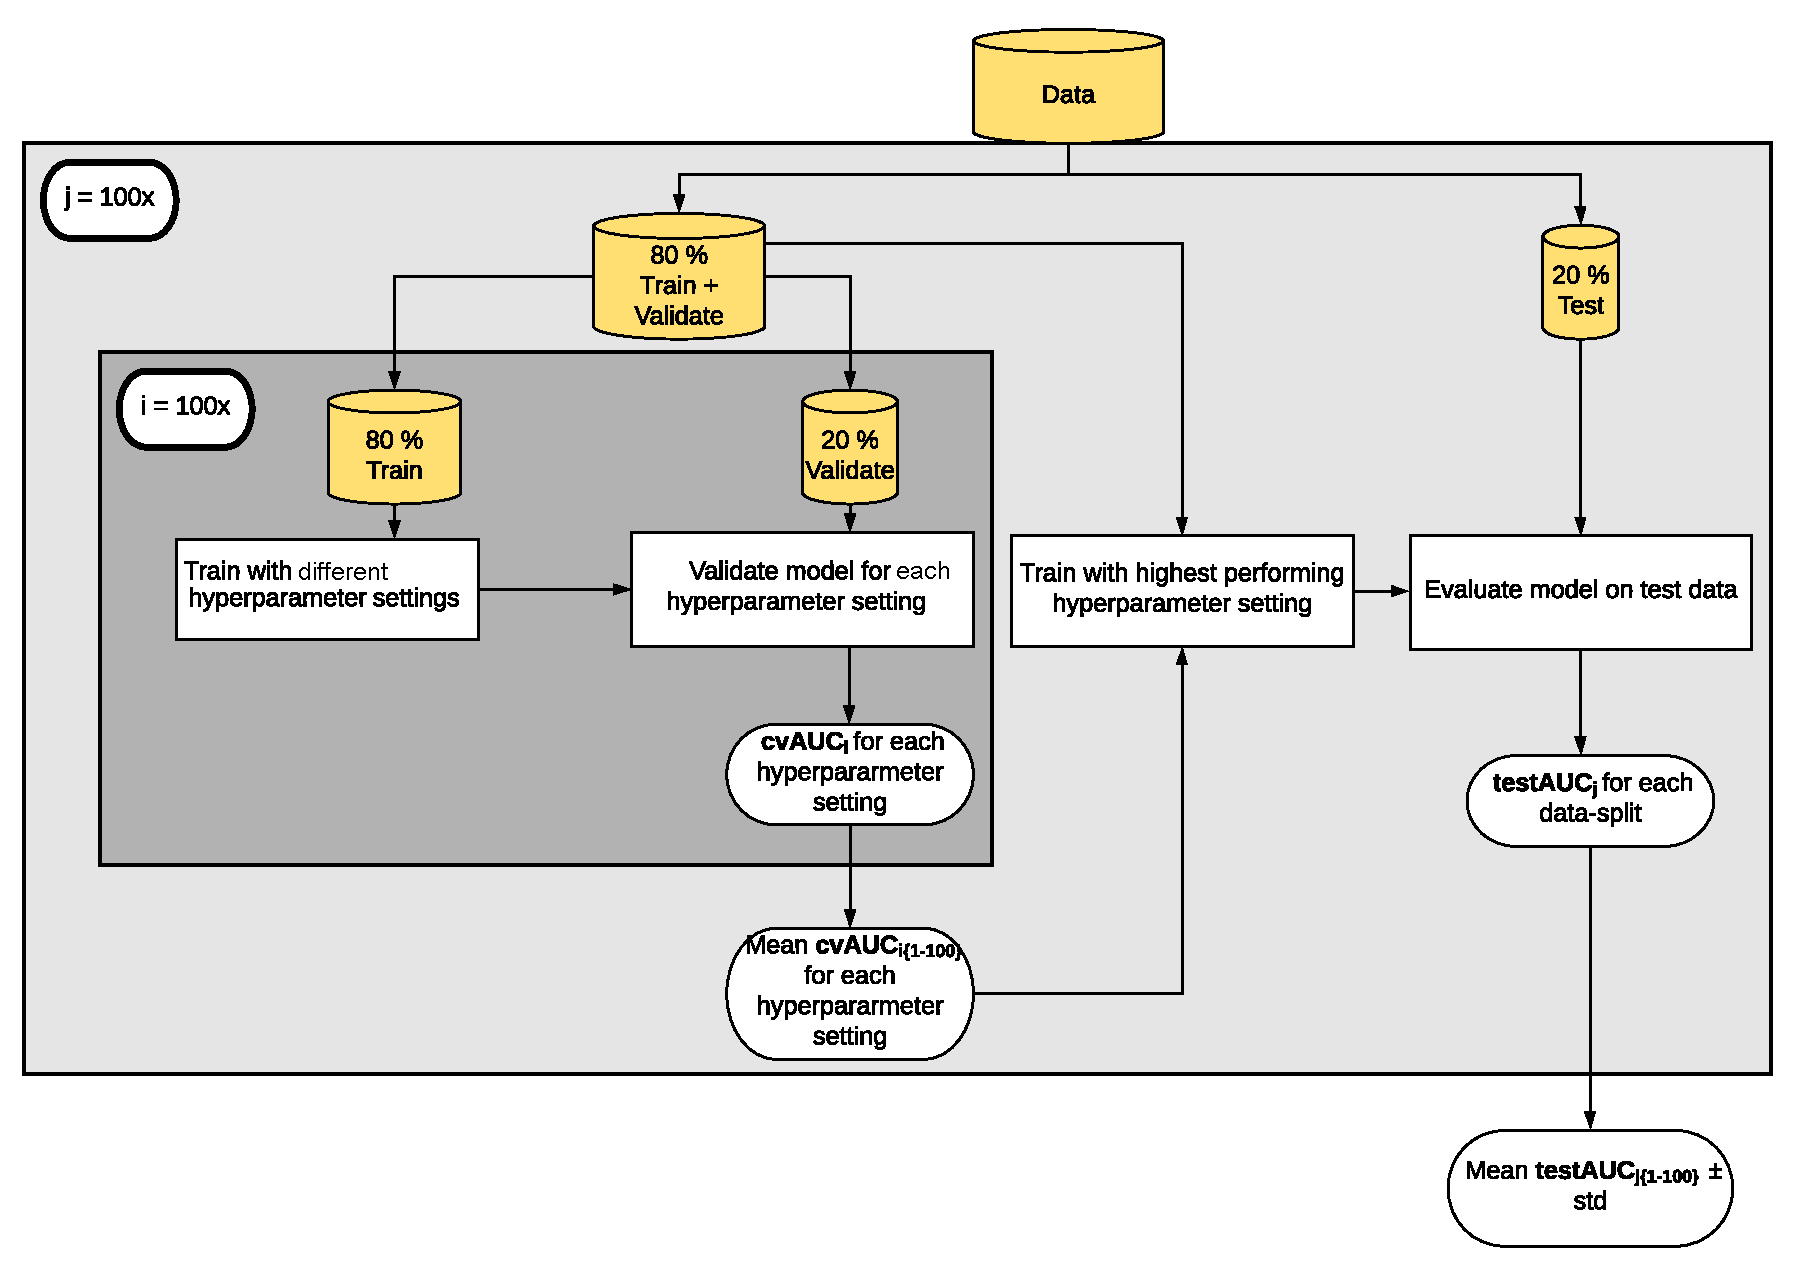
\includegraphics{Figure_1} \textbf{Figure 1. Machine learning pipeline
showing predictive model training and evaluation flowchart. } We split
the data 80\%/20\% stratified to maintain the overall label
distribution, performed five-fold cross-validation on the training data
to select the best hyperparameter setting and then using these
hyperparameters to train all of the training data. The model was
evaluated on a held-out set of data (not used in selecting the model).
Abbreviations: AUROC, area under the receiver operating characteristic
curve \newpage
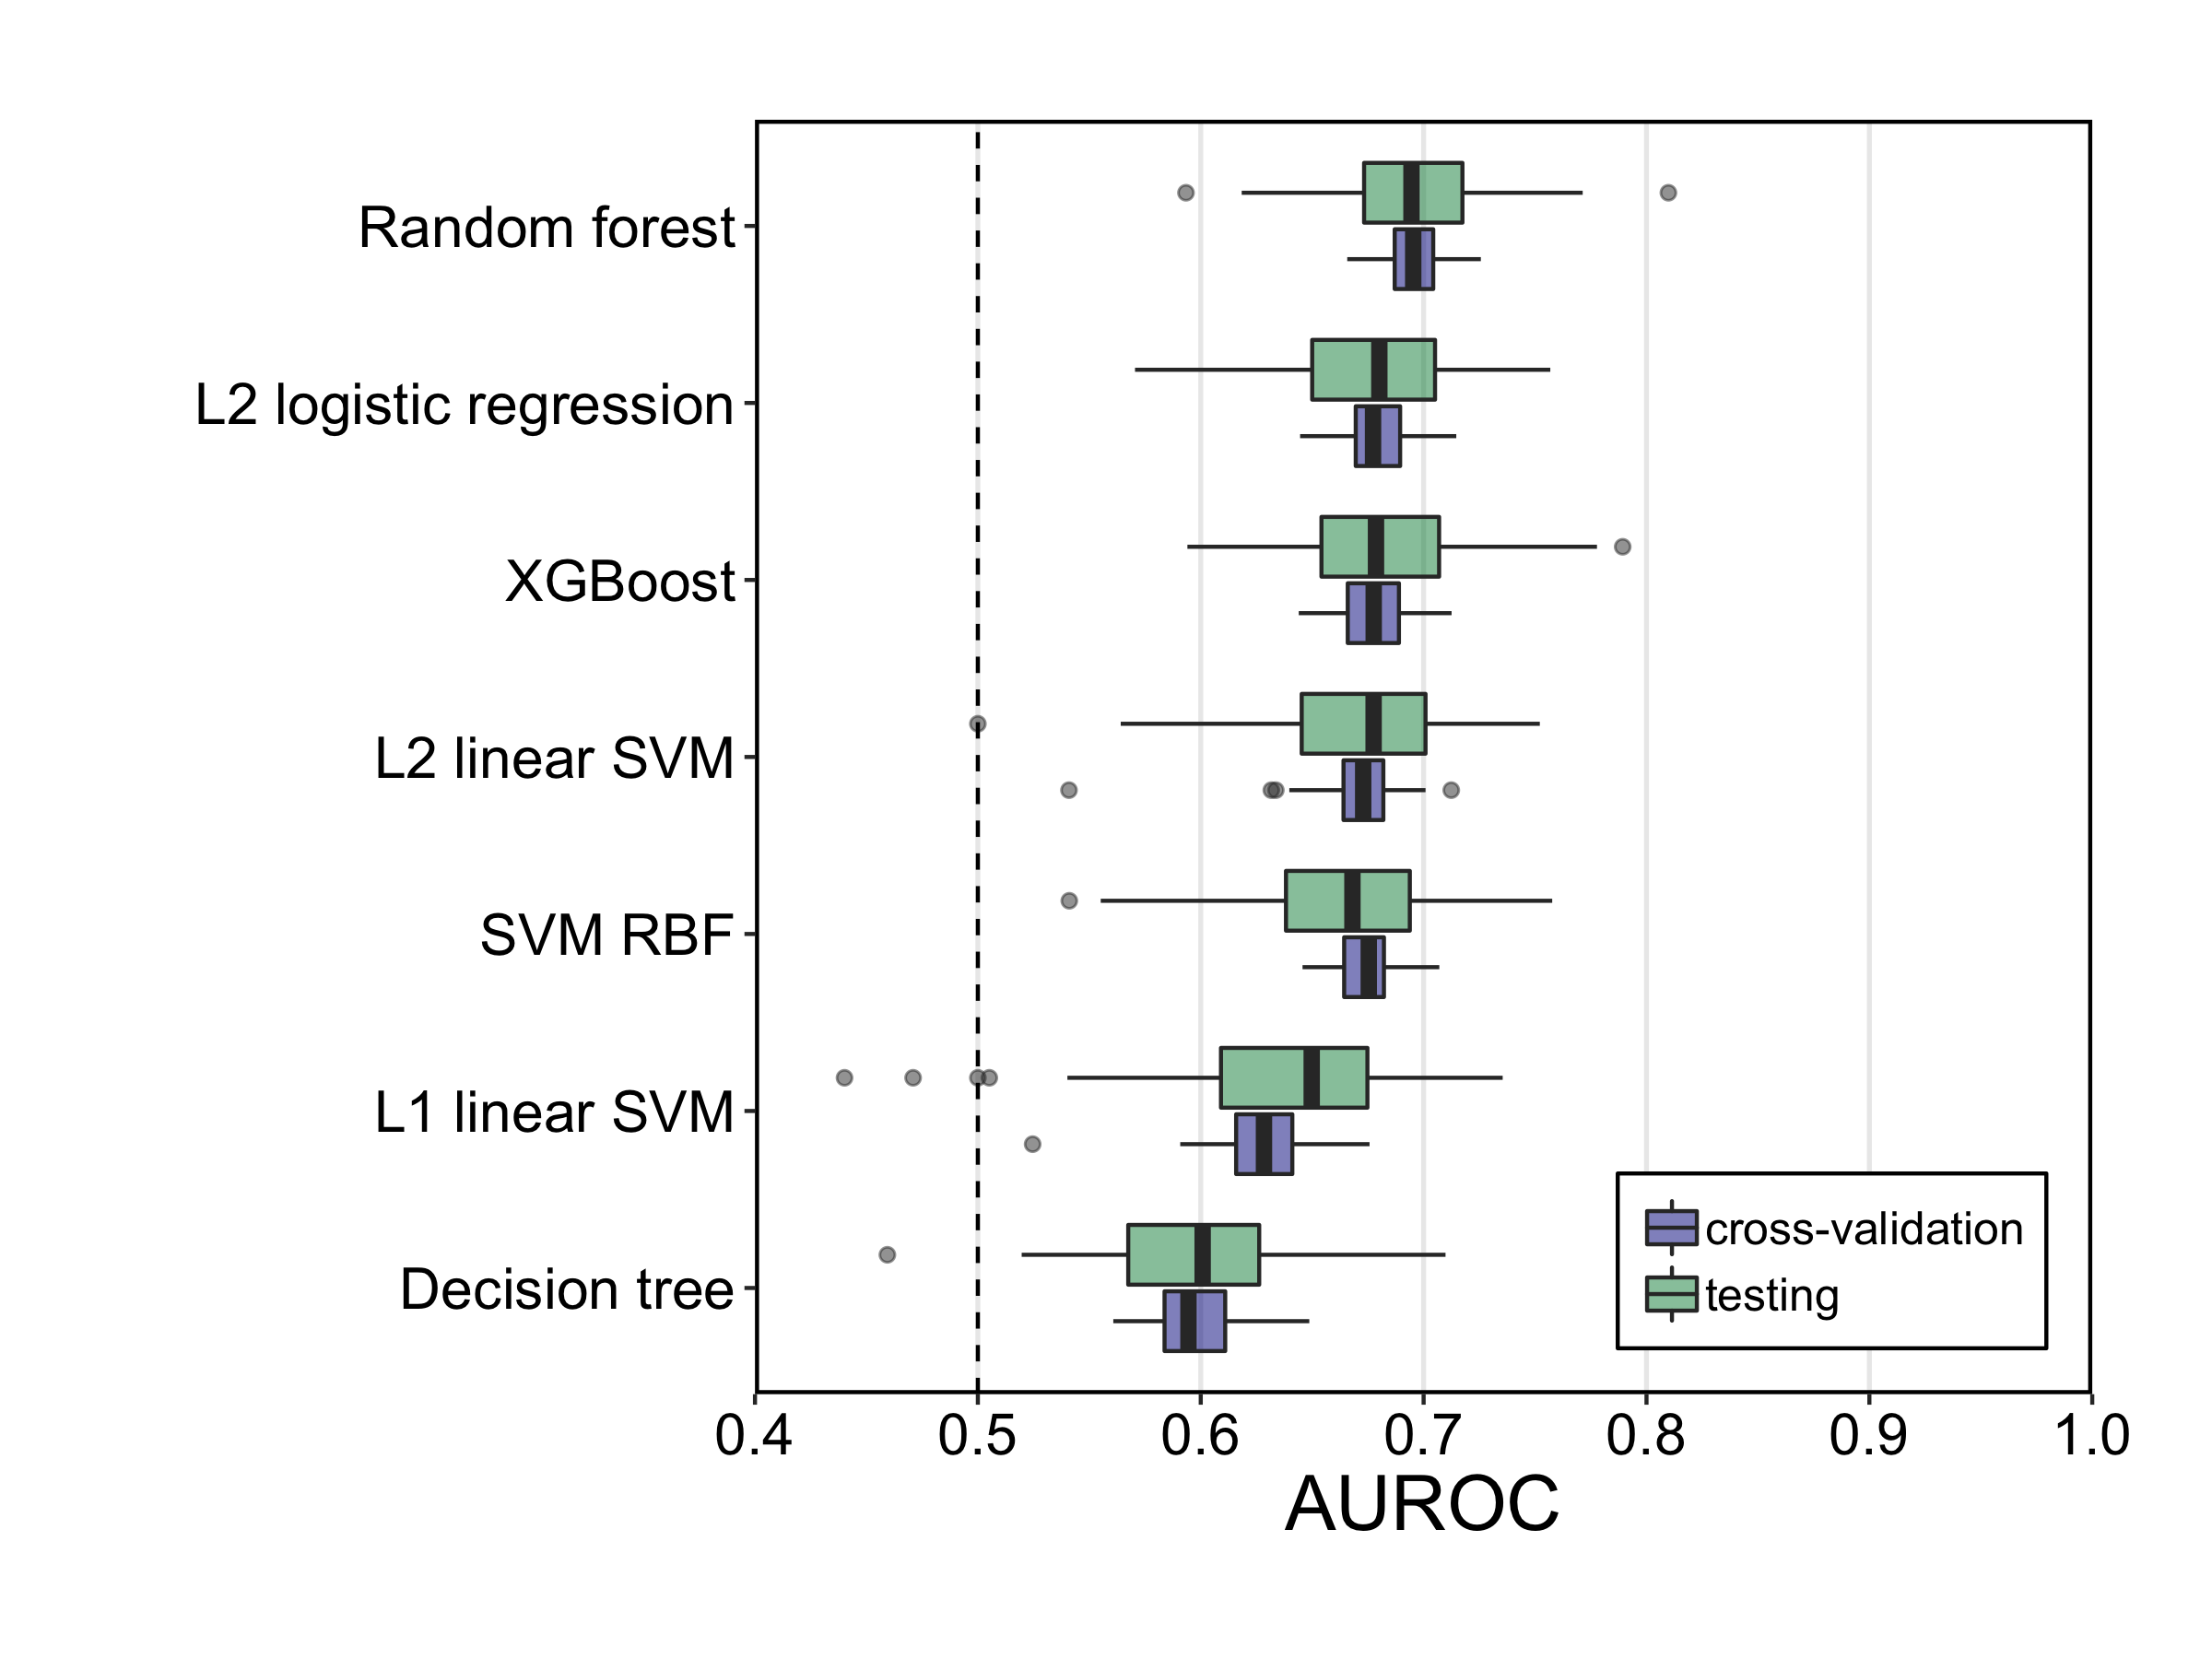
\includegraphics{Figure_2.png}

\textbf{Figure 2. Generalization and classification performance of ML
models using AUROC values of all cross validation and testing
performances. } The median AUROC for diagnosing individuals with SRN
using bacterial abundances was higher than chance (depicted by
horizontal line at 0.50) for all the ML models. Discriminative
performance of random forest model was higher than other ML models. The
boxplot shows quartiles at the box ends and the statistical median as
the horizontal line in the box. The whiskers show the farthest points
that are not outliers. Outliers are data points that are not within 3/2
times the interquartile ranges. Abbreviations: SRN, screen-relevant
neoplasias; AUROC, area under the receiver operating characteristic
curve; SVM, support vector machine; XGBoost, extreme gradient boosting
\newpage
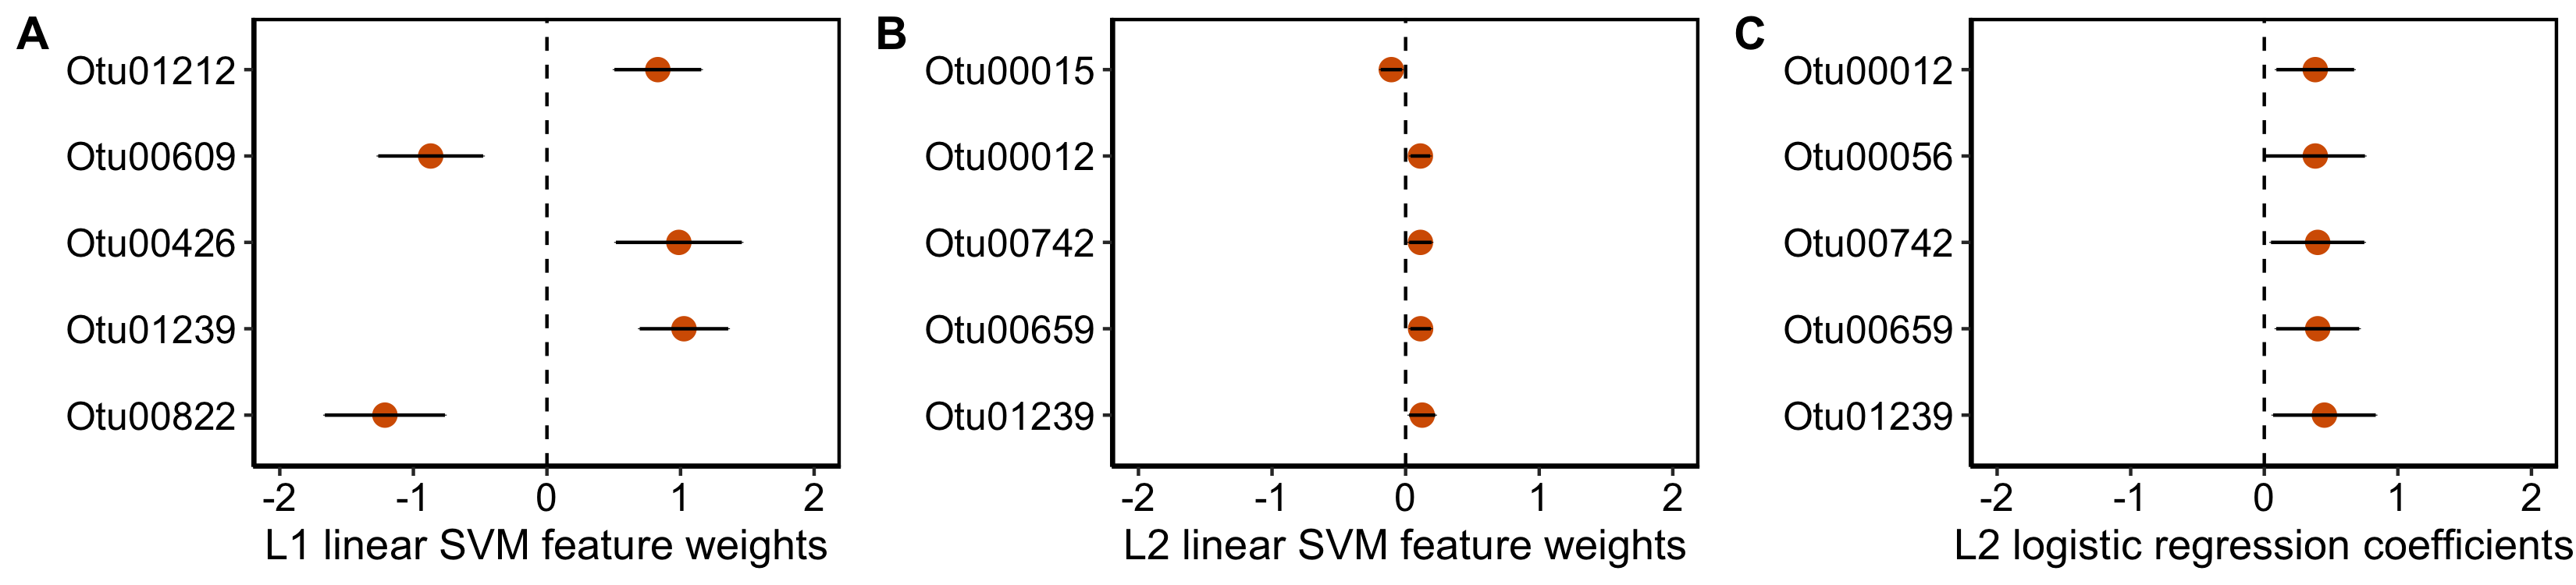
\includegraphics[height=15cm, width=10cm]{Figure_3.png}

\textbf{Figure 3. Interpretation of the linear ML models.} The absolute
feature weights of (A) L2 logistic regression coefficients (B) L1 SVM
with linear kernel (C) L2 SVM with linear kernel were ranked from
highest rank 1 to 100 for each data-split. The feature ranks of the
highest ranked five OTUs based on their median ranks are shown here.
Similar OTUs had the largest impact on the predictive performance of L2
logistic regression and L2 SVM with linear kernel. Abbreviations: SVM,
support vector machine; OTU, Operational Taxonomic Unit. \newpage
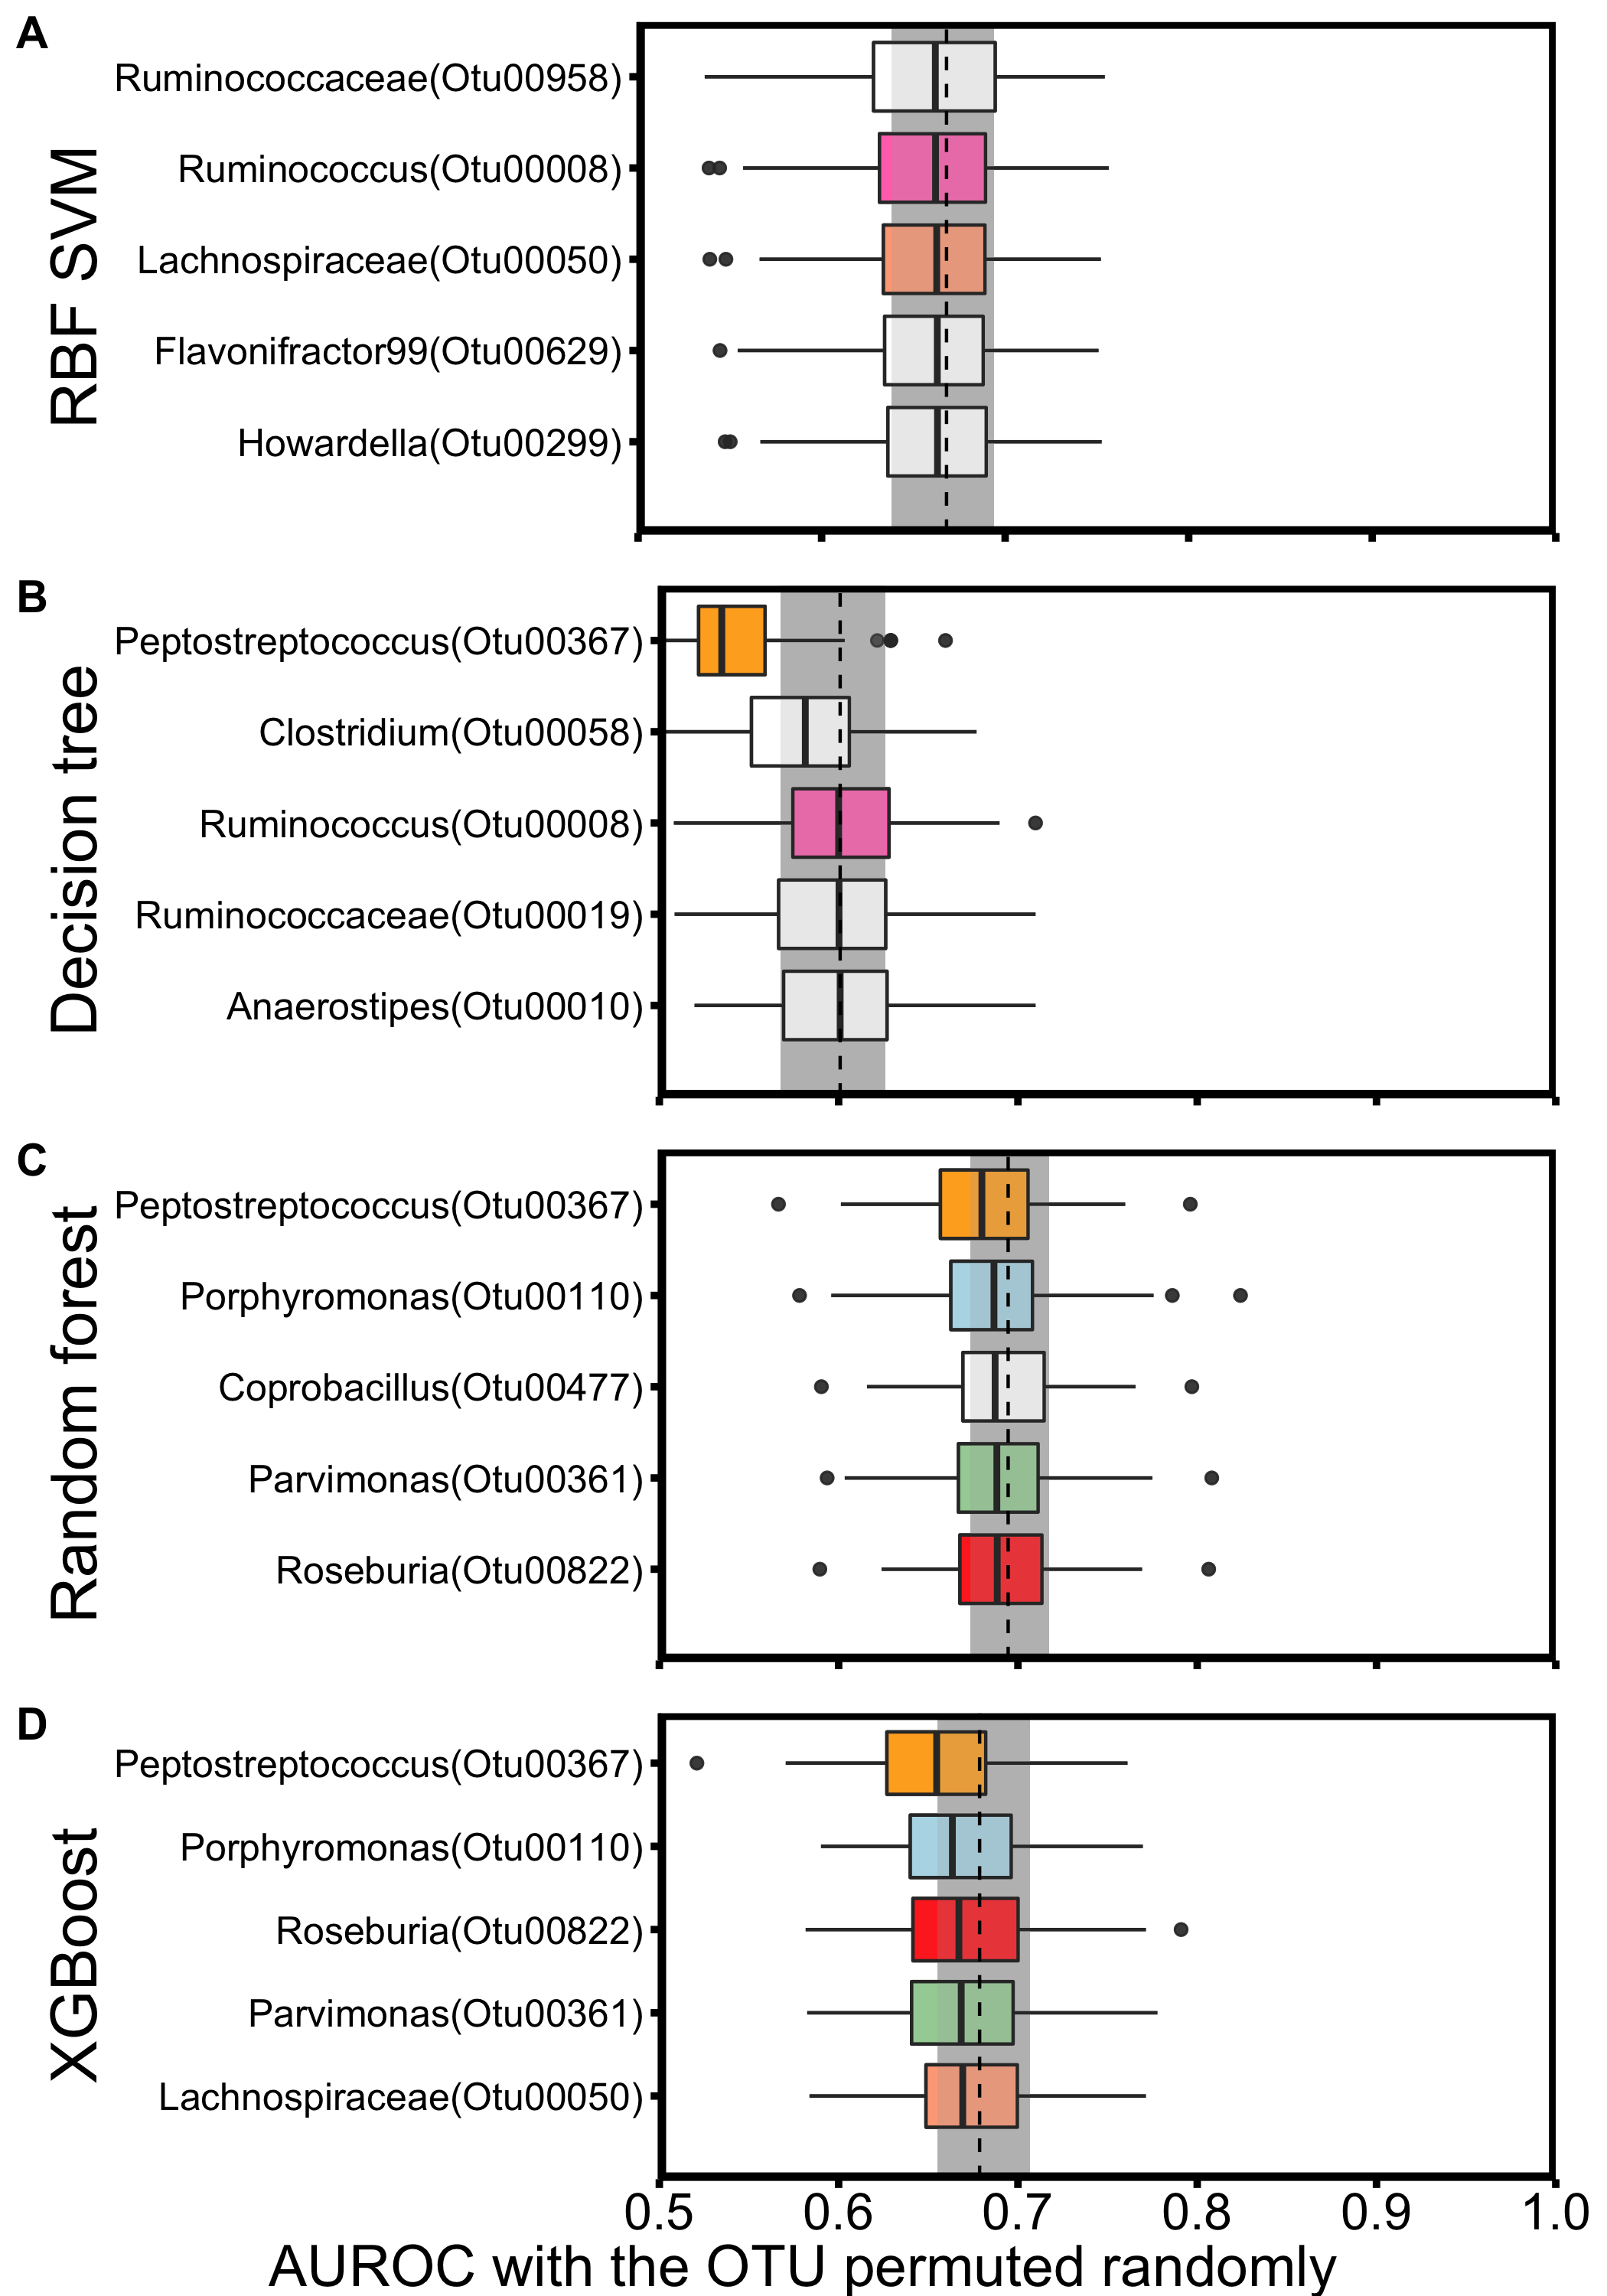
\includegraphics{Figure_4.png}

\textbf{Figure 4. Explanation of the non-linear ML models.} (A) SVM with
radial basis kernel (B) decision tree (C) random forest (D) XGboost
feaure importances were explanied using permutation importance using
held-out test set. The gray rectangle and the dashed line show the IQR
range and median of the base testing AUROC without any permutation
performed. The colors of the boxplots stand for the unique OTUs that are
shared among the different models; pink for OTU0008, salmon for OTU0050,
yellow for OTU00367, blue for OTU00110, green for OTU00361 and red for
OTU00882. For all the tree-based models, a \emph{Peptostreptococcus}
species (OTU00367) had the largest impact on predictive performance of
the model. Abbreviations: SVM, support vector machine; OTU, Operational
Taxonomic Unit; RBF, radial basis kernel; OTU, Operational Taxonomic
Unit. \newpage
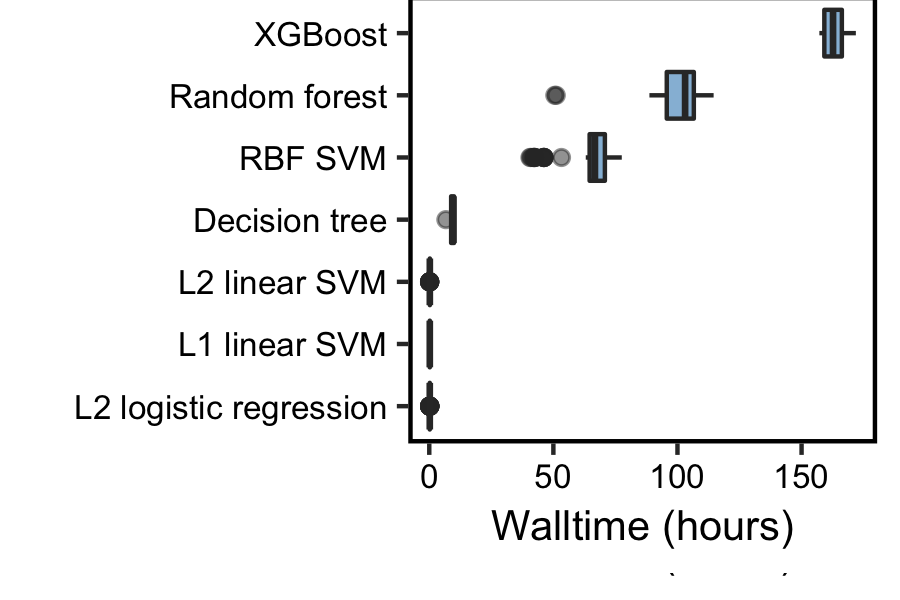
\includegraphics{Figure_5.png}

\textbf{Figure 5. Computational efficiency of seven ML models.} The
training times for of each data-split showed the differences in
computational efficieny of the seven models. The median training time in
hours was the highest for XGBoost and shortest for L1-regularized SVM
with linear kernel. The boxplot shows quartiles at the box ends and the
statistical median as the horizontal line in the box. The whiskers show
the farthest points that are not outliers. Outliers are data points that
are not within 3/2 times the interquartile ranges. Abbreviations: AUROC,
area under the receiver operating characteristic curve; SVM, support
vector machine; XGBoost, extreme gradient boosting.\\
\newpage
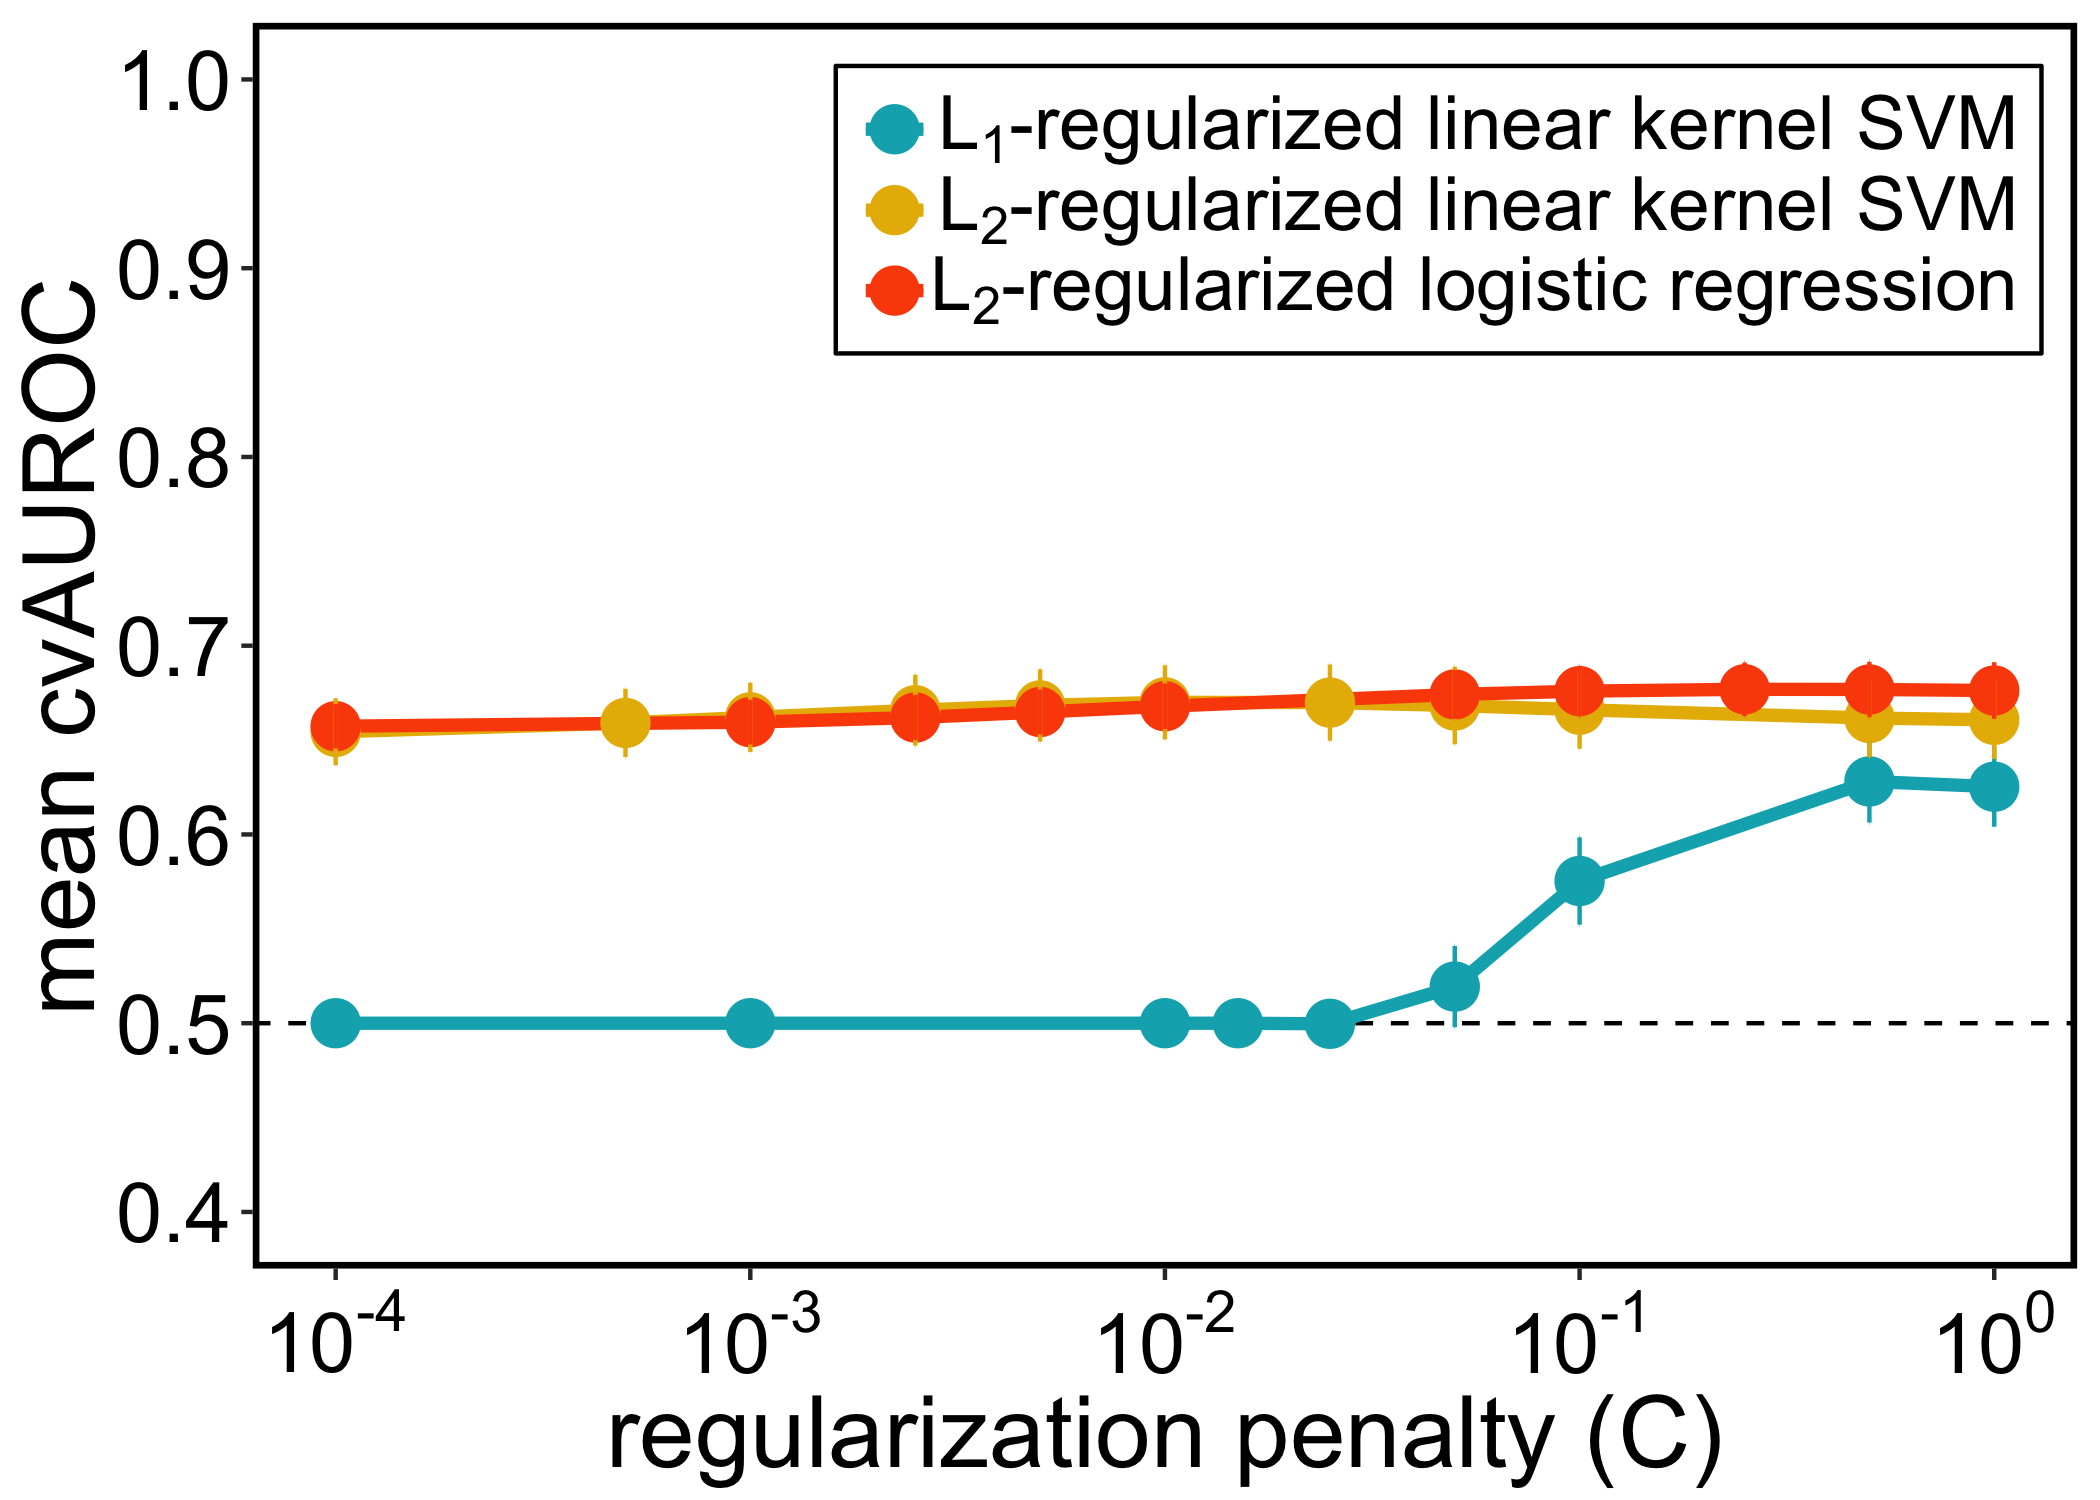
\includegraphics{Figure_S1.png}

\textbf{Figure S1. Hyperparameter setting performances for linear
models.} (A) L2 logistic regression (B) L1 SVM with linear kernel (C) L2
SVM with linear kernel mean cross-validation AUROC values when different
hyperparameters are used in training the model. The differences in AUROC
values when hyperparameters change show that hyperparameter tuning is a
crucial step in building a ML model.

\newpage

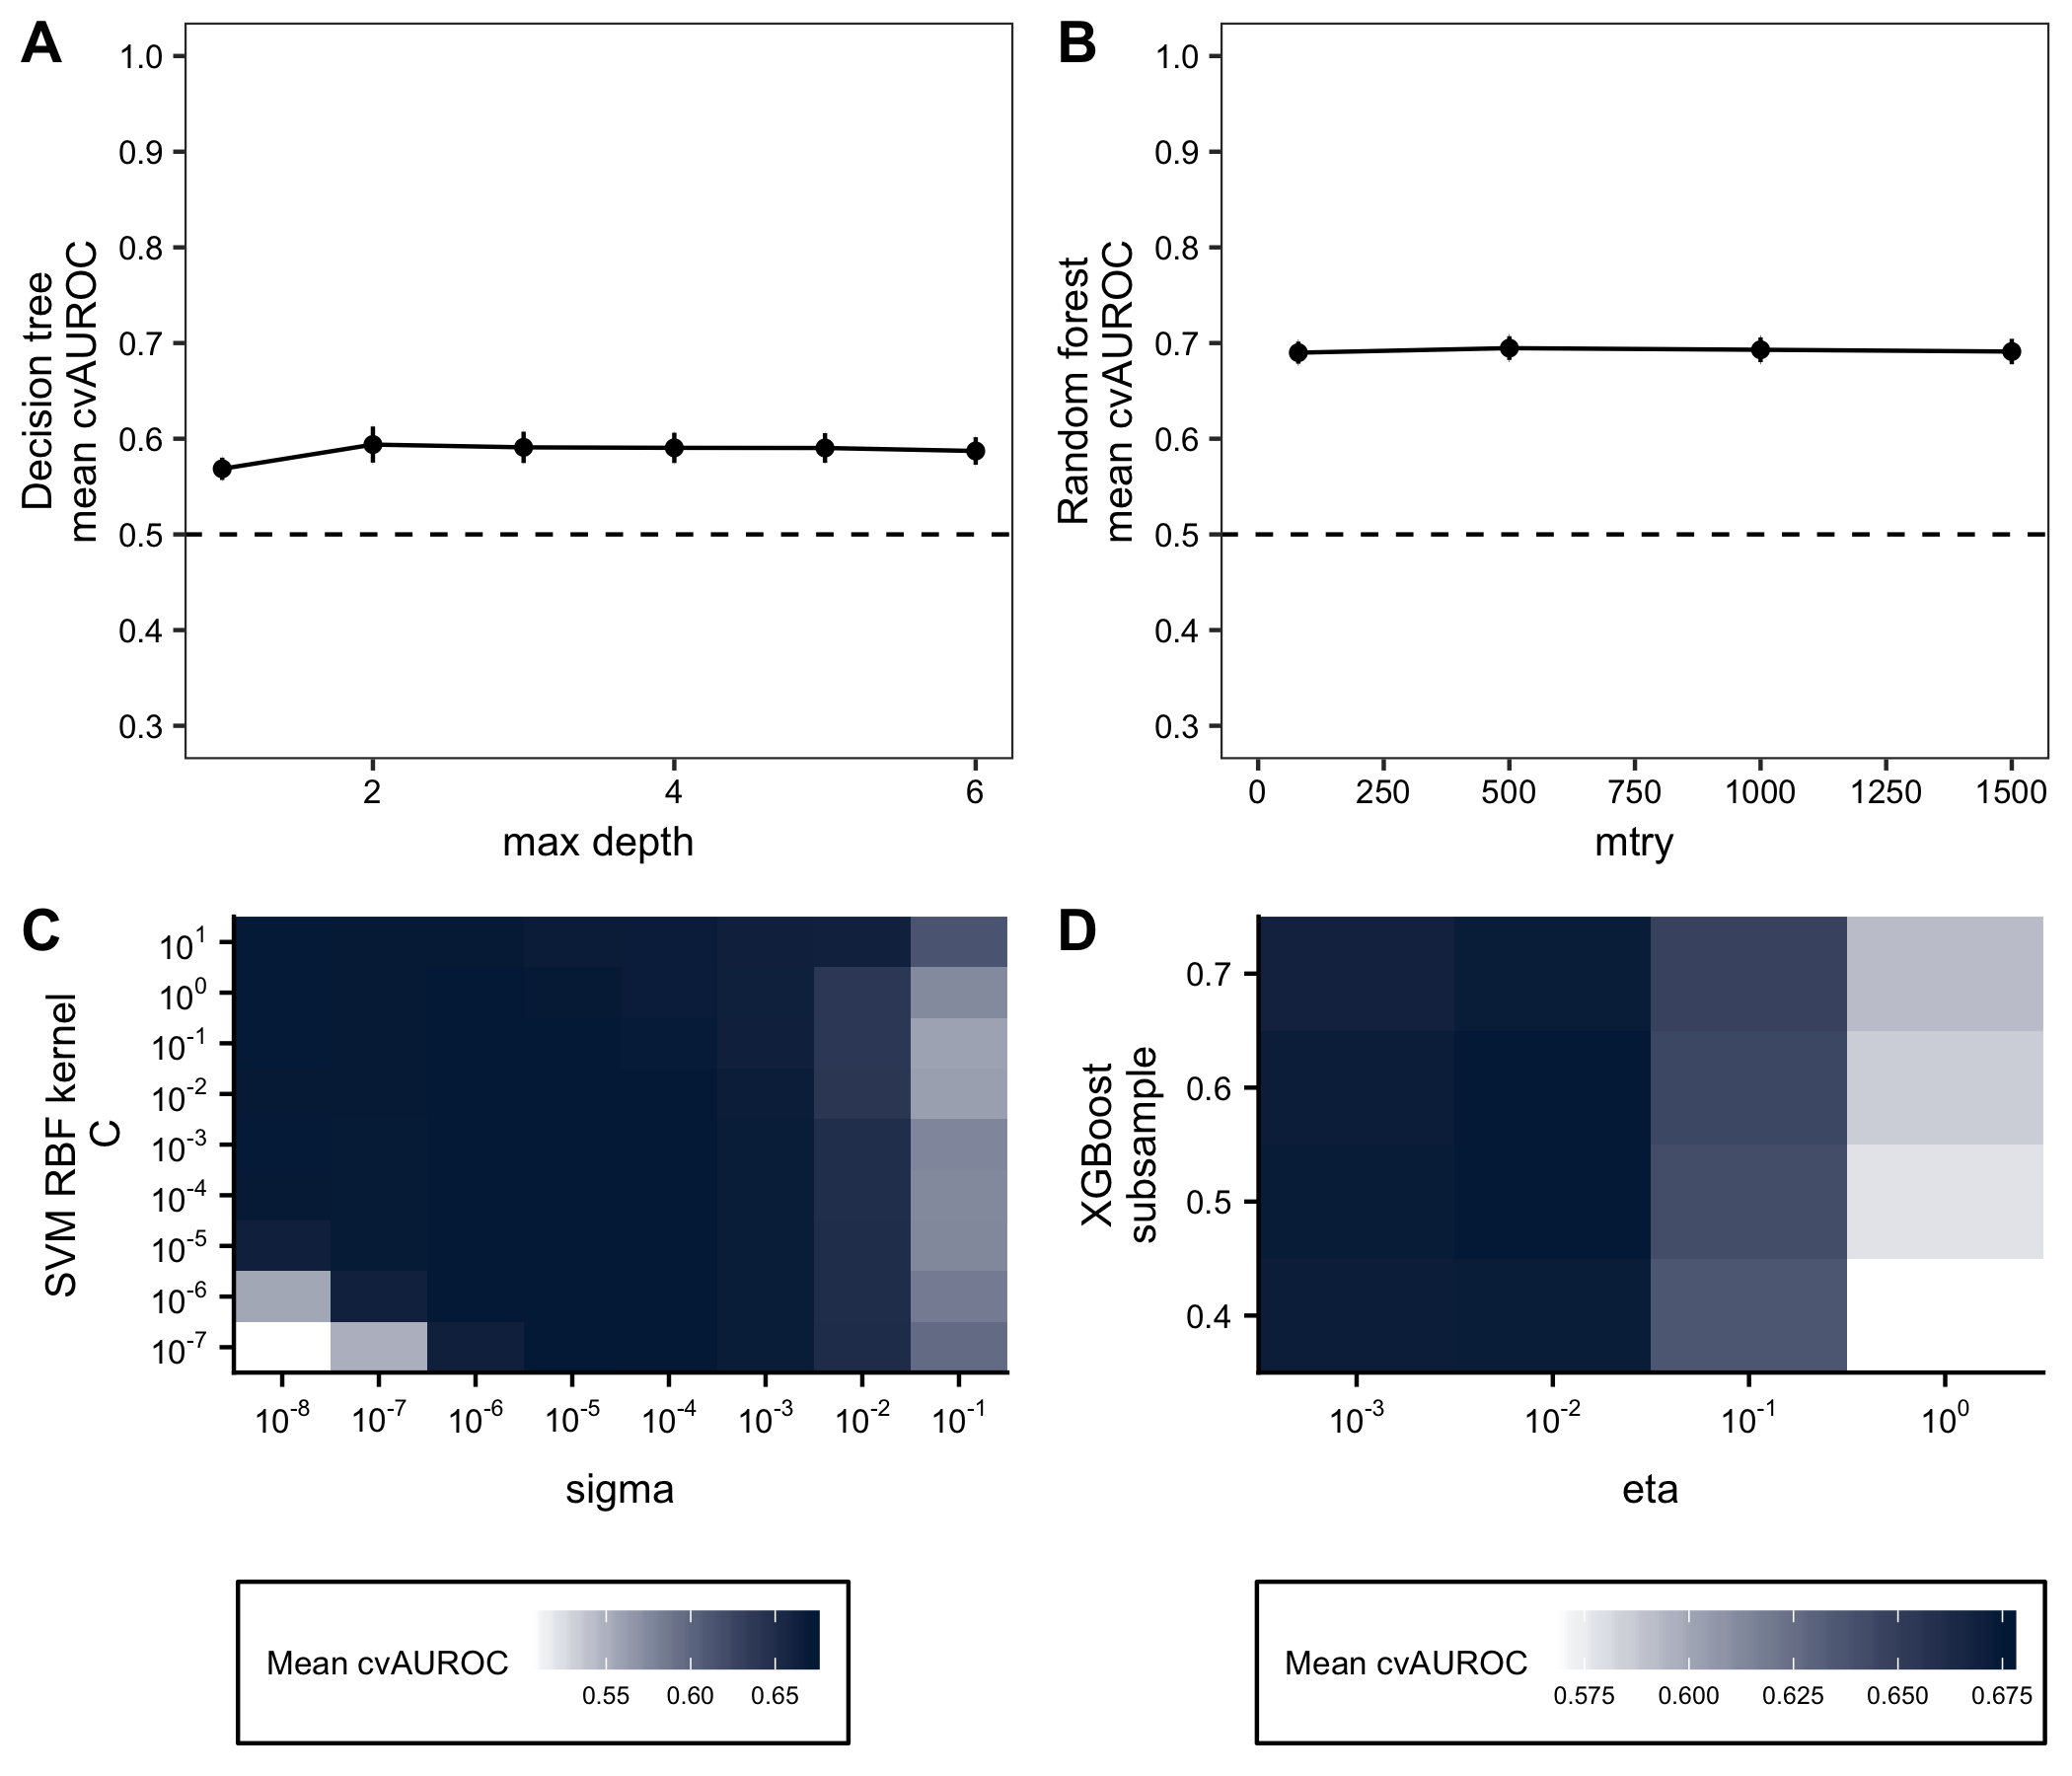
\includegraphics{Figure_S2.png}

\textbf{Figure S2. Hyperparameter setting performances for non-linear
models.} (A) Decision tree (B) Random forest (C) SVM with radial basis
kernel (D) XGoost mean cross-validation AUROC values when different
hyperparameters are used in training the model. The differences in AUROC
values when hyperparameters change show that hyperparameter tuning is a
crucial step in building a ML model. \newpage
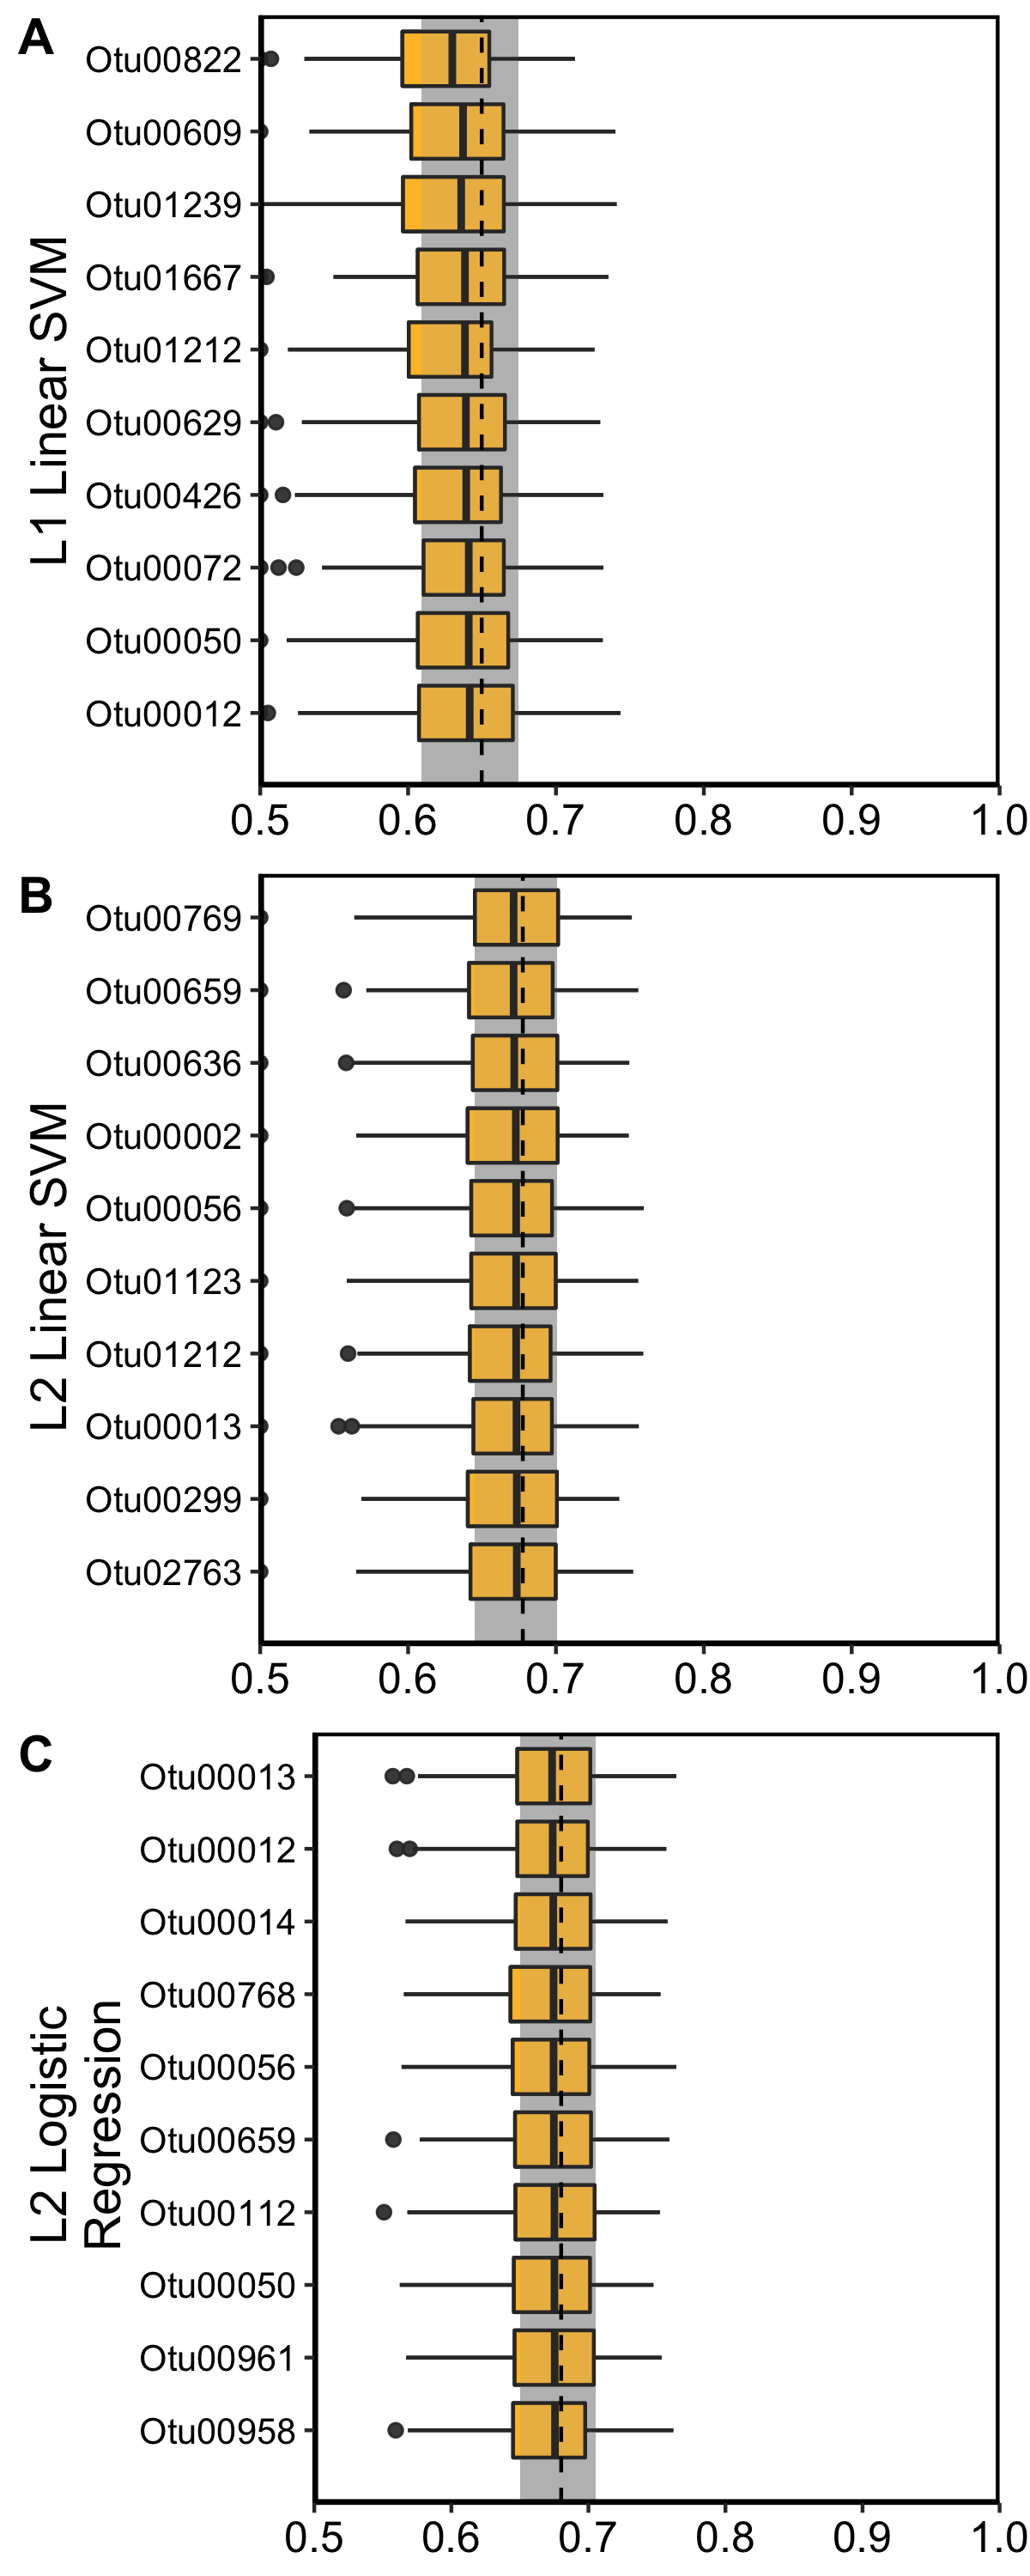
\includegraphics[height=17.5cm, width=13cm]{Figure_S4.png}

\textbf{Figure S3. Interpretation of the linear ML models with
permutation importance.} (A) L1-regularized SVM with linear kernel (B)
L2-regularized SVM with linear kernel and (C) L2-regularized logistic
regression were interpreted using permutation importance using held-out
test set. The gray rectangle and the dashed line show the IQR range and
median of the base testing AUROC without any permutation performed.
Abbreviations: SVM, support vector machine; OTU, Operational Taxonomic
Unit; RBF, radial basis kernel; OTU, Operational Taxonomic Unit.

\newpage

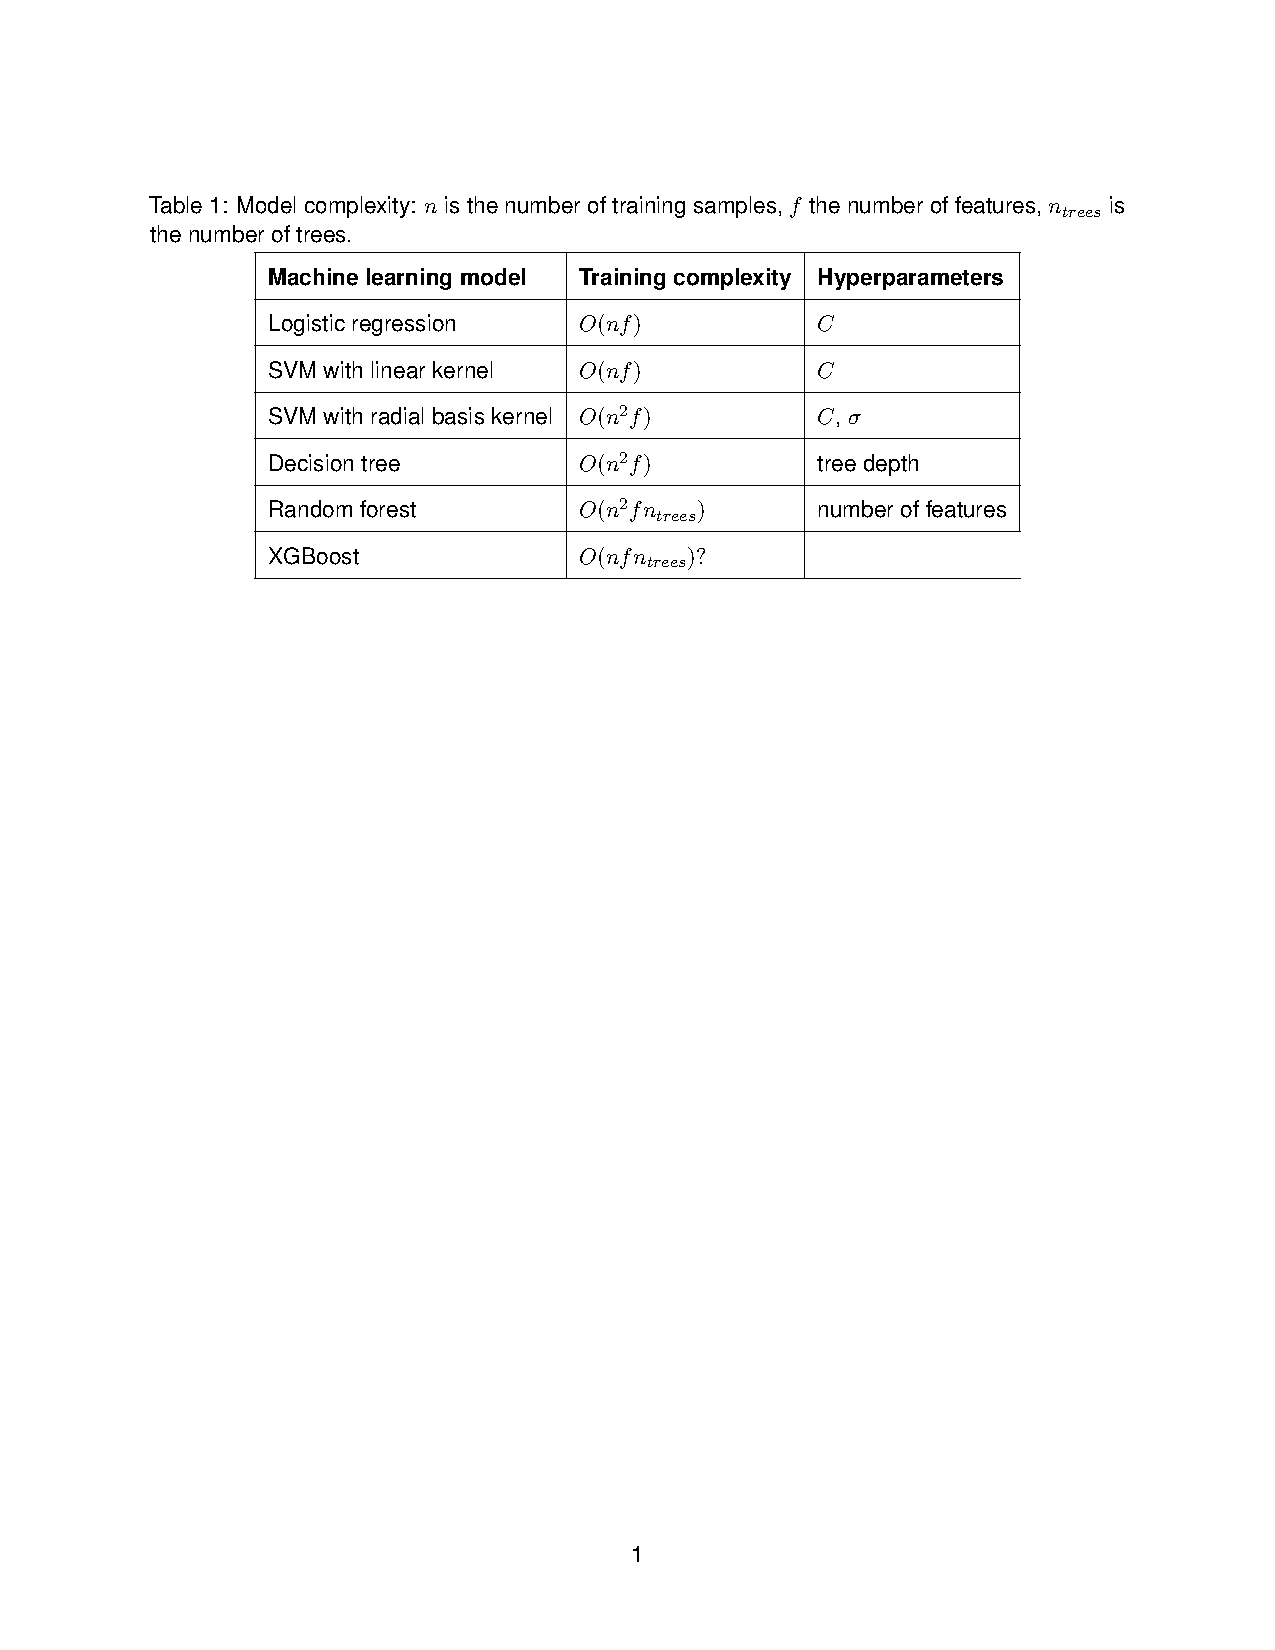
\includegraphics{TableS1.pdf} \textbf{Table S1. ML model complexity and
hyperparameter range.} \newpage

\subsection{References}\label{references}

\hypertarget{refs}{}
\hypertarget{ref-zeller_potential_2014}{}
1. \textbf{Zeller G}, \textbf{Tap J}, \textbf{Voigt AY},
\textbf{Sunagawa S}, \textbf{Kultima JR}, \textbf{Costea PI},
\textbf{Amiot A}, \textbf{Böhm J}, \textbf{Brunetti F},
\textbf{Habermann N}, \textbf{Hercog R}, \textbf{Koch M},
\textbf{Luciani A}, \textbf{Mende DR}, \textbf{Schneider MA},
\textbf{Schrotz-King P}, \textbf{Tournigand C}, \textbf{Tran Van Nhieu
J}, \textbf{Yamada T}, \textbf{Zimmermann J}, \textbf{Benes V},
\textbf{Kloor M}, \textbf{Ulrich CM}, \textbf{Knebel Doeberitz M von},
\textbf{Sobhani I}, \textbf{Bork P}. 2014. Potential of fecal microbiota
for early-stage detection of colorectal cancer. Mol Syst Biol
\textbf{10}.
doi:\href{https://doi.org/10.15252/msb.20145645}{10.15252/msb.20145645}.

\hypertarget{ref-zackular_human_2014}{}
2. \textbf{Zackular JP}, \textbf{Rogers MAM}, \textbf{Ruffin MT},
\textbf{Schloss PD}. 2014. The human gut microbiome as a screening tool
for colorectal cancer. Cancer Prev Res \textbf{7}:1112--1121.
doi:\href{https://doi.org/10.1158/1940-6207.CAPR-14-0129}{10.1158/1940-6207.CAPR-14-0129}.

\hypertarget{ref-baxter_dna_2016}{}
3. \textbf{Baxter NT}, \textbf{Koumpouras CC}, \textbf{Rogers MAM},
\textbf{Ruffin MT}, \textbf{Schloss PD}. 2016. DNA from fecal
immunochemical test can replace stool for detection of colonic lesions
using a microbiota-based model. Microbiome \textbf{4}.
doi:\href{https://doi.org/10.1186/s40168-016-0205-y}{10.1186/s40168-016-0205-y}.

\hypertarget{ref-baxter_microbiota-based_2016}{}
4. \textbf{Baxter NT}, \textbf{Ruffin MT}, \textbf{Rogers MAM},
\textbf{Schloss PD}. 2016. Microbiota-based model improves the
sensitivity of fecal immunochemical test for detecting colonic lesions.
Genome Medicine \textbf{8}:37.
doi:\href{https://doi.org/10.1186/s13073-016-0290-3}{10.1186/s13073-016-0290-3}.

\hypertarget{ref-hale_shifts_2017}{}
5. \textbf{Hale VL}, \textbf{Chen J}, \textbf{Johnson S},
\textbf{Harrington SC}, \textbf{Yab TC}, \textbf{Smyrk TC},
\textbf{Nelson H}, \textbf{Boardman LA}, \textbf{Druliner BR},
\textbf{Levin TR}, \textbf{Rex DK}, \textbf{Ahnen DJ}, \textbf{Lance P},
\textbf{Ahlquist DA}, \textbf{Chia N}. 2017. Shifts in the fecal
microbiota associated with adenomatous polyps. Cancer Epidemiol
Biomarkers Prev \textbf{26}:85--94.
doi:\href{https://doi.org/10.1158/1055-9965.EPI-16-0337}{10.1158/1055-9965.EPI-16-0337}.

\hypertarget{ref-pasolli_machine_2016}{}
6. \textbf{Pasolli E}, \textbf{Truong DT}, \textbf{Malik F},
\textbf{Waldron L}, \textbf{Segata N}. 2016. Machine learning
meta-analysis of large metagenomic datasets: Tools and biological
insights. PLoS Comput Biol \textbf{12}.
doi:\href{https://doi.org/10.1371/journal.pcbi.1004977}{10.1371/journal.pcbi.1004977}.

\hypertarget{ref-sze_looking_2016}{}
7. \textbf{Sze MA}, \textbf{Schloss PD}. 2016. Looking for a signal in
the noise: Revisiting obesity and the microbiome. mBio \textbf{7}.
doi:\href{https://doi.org/10.1128/mBio.01018-16}{10.1128/mBio.01018-16}.

\hypertarget{ref-walters_meta-analyses_2014}{}
8. \textbf{Walters WA}, \textbf{Xu Z}, \textbf{Knight R}. 2014.
Meta-analyses of human gut microbes associated with obesity and IBD.
FEBS Lett \textbf{588}:4223--4233.
doi:\href{https://doi.org/10.1016/j.febslet.2014.09.039}{10.1016/j.febslet.2014.09.039}.

\hypertarget{ref-vazquez-baeza_guiding_2018}{}
9. \textbf{Vázquez-Baeza Y}, \textbf{Gonzalez A}, \textbf{Xu ZZ},
\textbf{Washburne A}, \textbf{Herfarth HH}, \textbf{Sartor RB},
\textbf{Knight R}. 2018. Guiding longitudinal sampling in IBD cohorts.
Gut \textbf{67}:1743--1745.
doi:\href{https://doi.org/10.1136/gutjnl-2017-315352}{10.1136/gutjnl-2017-315352}.

\hypertarget{ref-qin_alterations_2014}{}
10. \textbf{Qin N}, \textbf{Yang F}, \textbf{Li A}, \textbf{Prifti E},
\textbf{Chen Y}, \textbf{Shao L}, \textbf{Guo J}, \textbf{Le Chatelier
E}, \textbf{Yao J}, \textbf{Wu L}, \textbf{Zhou J}, \textbf{Ni S},
\textbf{Liu L}, \textbf{Pons N}, \textbf{Batto JM}, \textbf{Kennedy SP},
\textbf{Leonard P}, \textbf{Yuan C}, \textbf{Ding W}, \textbf{Chen Y},
\textbf{Hu X}, \textbf{Zheng B}, \textbf{Qian G}, \textbf{Xu W},
\textbf{Ehrlich SD}, \textbf{Zheng S}, \textbf{Li L}. 2014. Alterations
of the human gut microbiome in liver cirrhosis. Nature
\textbf{513}:59--64.
doi:\href{https://doi.org/10.1038/nature13568}{10.1038/nature13568}.

\hypertarget{ref-geman_deep_2018}{}
11. \textbf{Geman O}, \textbf{Chiuchisan I}, \textbf{Covasa M},
\textbf{Doloc C}, \textbf{Milici M-R}, \textbf{Milici L-D}. 2018. Deep
learning tools for human microbiome big data, pp. 265--275. \emph{In}
Balas, VE, Jain, LC, Balas, MM (eds.), Soft computing applications.
Springer International Publishing.

\hypertarget{ref-thaiss_persistent_2016}{}
12. \textbf{Thaiss CA}, \textbf{Itav S}, \textbf{Rothschild D},
\textbf{Meijer MT}, \textbf{Levy M}, \textbf{Moresi C},
\textbf{Dohnalová L}, \textbf{Braverman S}, \textbf{Rozin S},
\textbf{Malitsky S}, \textbf{Dori-Bachash M}, \textbf{Kuperman Y},
\textbf{Biton I}, \textbf{Gertler A}, \textbf{Harmelin A},
\textbf{Shapiro H}, \textbf{Halpern Z}, \textbf{Aharoni A},
\textbf{Segal E}, \textbf{Elinav E}. 2016. Persistent microbiome
alterations modulate the rate of post-dieting weight regain. Nature
\textbf{540}:544--551.
doi:\href{https://doi.org/10.1038/nature20796}{10.1038/nature20796}.

\hypertarget{ref-dadkhah_gut_2019}{}
13. \textbf{Dadkhah E}, \textbf{Sikaroodi M}, \textbf{Korman L},
\textbf{Hardi R}, \textbf{Baybick J}, \textbf{Hanzel D}, \textbf{Kuehn
G}, \textbf{Kuehn T}, \textbf{Gillevet PM}. 2019. Gut microbiome
identifies risk for colorectal polyps. BMJ Open Gastroenterology
\textbf{6}:e000297.
doi:\href{https://doi.org/10.1136/bmjgast-2019-000297}{10.1136/bmjgast-2019-000297}.

\hypertarget{ref-flemer_oral_2018}{}
14. \textbf{Flemer B}, \textbf{Warren RD}, \textbf{Barrett MP},
\textbf{Cisek K}, \textbf{Das A}, \textbf{Jeffery IB}, \textbf{Hurley
E}, \textbf{O`Riordain M}, \textbf{Shanahan F}, \textbf{O`Toole PW}.
2018. The oral microbiota in colorectal cancer is distinctive and
predictive. Gut \textbf{67}:1454--1463.
doi:\href{https://doi.org/10.1136/gutjnl-2017-314814}{10.1136/gutjnl-2017-314814}.

\hypertarget{ref-dai_multi-cohort_2018}{}
15. \textbf{Dai Z}, \textbf{Coker OO}, \textbf{Nakatsu G}, \textbf{Wu
WKK}, \textbf{Zhao L}, \textbf{Chen Z}, \textbf{Chan FKL},
\textbf{Kristiansen K}, \textbf{Sung JJY}, \textbf{Wong SH}, \textbf{Yu
J}. 2018. Multi-cohort analysis of colorectal cancer metagenome
identified altered bacteria across populations and universal bacterial
markers. Microbiome \textbf{6}:70.
doi:\href{https://doi.org/10.1186/s40168-018-0451-2}{10.1186/s40168-018-0451-2}.

\hypertarget{ref-montassier_pretreatment_2016}{}
16. \textbf{Montassier E}, \textbf{Al-Ghalith GA}, \textbf{Ward T},
\textbf{Corvec S}, \textbf{Gastinne T}, \textbf{Potel G}, \textbf{Moreau
P}, \textbf{Cochetiere MF de la}, \textbf{Batard E}, \textbf{Knights D}.
2016. Pretreatment gut microbiome predicts chemotherapy-related
bloodstream infection. Genome Medicine \textbf{8}:49.
doi:\href{https://doi.org/10.1186/s13073-016-0301-4}{10.1186/s13073-016-0301-4}.

\hypertarget{ref-papa_non-invasive_2012}{}
17. \textbf{Papa E}, \textbf{Docktor M}, \textbf{Smillie C},
\textbf{Weber S}, \textbf{Preheim SP}, \textbf{Gevers D},
\textbf{Giannoukos G}, \textbf{Ciulla D}, \textbf{Tabbaa D},
\textbf{Ingram J}, \textbf{Schauer DB}, \textbf{Ward DV},
\textbf{Korzenik JR}, \textbf{Xavier RJ}, \textbf{Bousvaros A},
\textbf{Alm EJ}. 2012. Non-invasive mapping of the gastrointestinal
microbiota identifies children with inflammatory bowel disease. PLOS ONE
\textbf{7}:e39242.
doi:\href{https://doi.org/10.1371/journal.pone.0039242}{10.1371/journal.pone.0039242}.

\hypertarget{ref-mossotto_classification_2017}{}
18. \textbf{Mossotto E}, \textbf{Ashton JJ}, \textbf{Coelho T},
\textbf{Beattie RM}, \textbf{MacArthur BD}, \textbf{Ennis S}. 2017.
Classification of paediatric inflammatory bowel disease using machine
learning. Scientific Reports \textbf{7}.
doi:\href{https://doi.org/10.1038/s41598-017-02606-2}{10.1038/s41598-017-02606-2}.

\hypertarget{ref-ai_systematic_2017}{}
19. \textbf{Ai L}, \textbf{Tian H}, \textbf{Chen Z}, \textbf{Chen H},
\textbf{Xu J}, \textbf{Fang J-Y}. 2017. Systematic evaluation of
supervised classifiers for fecal microbiota-based prediction of
colorectal cancer. Oncotarget \textbf{8}:9546--9556.
doi:\href{https://doi.org/10.18632/oncotarget.14488}{10.18632/oncotarget.14488}.

\hypertarget{ref-wong_quantitation_2017}{}
20. \textbf{Wong SH}, \textbf{Kwong TNY}, \textbf{Chow T-C}, \textbf{Luk
AKC}, \textbf{Dai RZW}, \textbf{Nakatsu G}, \textbf{Lam TYT},
\textbf{Zhang L}, \textbf{Wu JCY}, \textbf{Chan FKL}, \textbf{Ng SSM},
\textbf{Wong MCS}, \textbf{Ng SC}, \textbf{Wu WKK}, \textbf{Yu J},
\textbf{Sung JJY}. 2017. Quantitation of faecal fusobacterium improves
faecal immunochemical test in detecting advanced colorectal neoplasia.
Gut \textbf{66}:1441--1448.
doi:\href{https://doi.org/10.1136/gutjnl-2016-312766}{10.1136/gutjnl-2016-312766}.

\hypertarget{ref-galkin_human_2018}{}
21. \textbf{Galkin F}, \textbf{Aliper A}, \textbf{Putin E},
\textbf{Kuznetsov I}, \textbf{Gladyshev VN}, \textbf{Zhavoronkov A}.
2018. Human microbiome aging clocks based on deep learning and tandem of
permutation feature importance and accumulated local effects. bioRxiv.
doi:\href{https://doi.org/10.1101/507780}{10.1101/507780}.

\hypertarget{ref-reiman_using_2017}{}
22. \textbf{Reiman D}, \textbf{Metwally A}, \textbf{Dai Y}. 2017. Using
convolutional neural networks to explore the microbiome, pp. 4269--4272.
\emph{In} 2017 39th annual international conference of the IEEE
engineering in medicine and biology society (EMBC).

\hypertarget{ref-fioravanti_phylogenetic_2017}{}
23. \textbf{Fioravanti D}, \textbf{Giarratano Y}, \textbf{Maggio V},
\textbf{Agostinelli C}, \textbf{Chierici M}, \textbf{Jurman G},
\textbf{Furlanello C}. 2017. Phylogenetic convolutional neural networks
in metagenomics. arXiv:170902268 {[}cs, q-bio{]}.

\hypertarget{ref-rudin_please_2018}{}
24. \textbf{Rudin C}. 2018. Please stop explaining black box models for
high stakes decisions. arXiv:181110154 {[}cs, stat{]}.

\hypertarget{ref-rudin_optimized_2018}{}
25. \textbf{Rudin C}, \textbf{Ustun B}. 2018. Optimized scoring systems:
Toward trust in machine learning for healthcare and criminal justice.
Interfaces \textbf{48}:449--466.
doi:\href{https://doi.org/10.1287/inte.2018.0957}{10.1287/inte.2018.0957}.

\hypertarget{ref-knights_human-associated_2011}{}
26. \textbf{Knights D}, \textbf{Parfrey LW}, \textbf{Zaneveld J},
\textbf{Lozupone C}, \textbf{Knight R}. 2011. Human-associated microbial
signatures: Examining their predictive value. Cell Host Microbe
\textbf{10}:292--296.
doi:\href{https://doi.org/10.1016/j.chom.2011.09.003}{10.1016/j.chom.2011.09.003}.

\hypertarget{ref-sze_leveraging_2018}{}
27. \textbf{Sze MA}, \textbf{Schloss PD}. 2018. Leveraging existing 16S
rRNA gene surveys to identify reproducible biomarkers in individuals
with colorectal tumors. mBio \textbf{9}:e00630--18.
doi:\href{https://doi.org/10.1128/mBio.00630-18}{10.1128/mBio.00630-18}.

\hypertarget{ref-schloss_introducing_2009}{}
28. \textbf{Schloss PD}, \textbf{Westcott SL}, \textbf{Ryabin T},
\textbf{Hall JR}, \textbf{Hartmann M}, \textbf{Hollister EB},
\textbf{Lesniewski RA}, \textbf{Oakley BB}, \textbf{Parks DH},
\textbf{Robinson CJ}, \textbf{Sahl JW}, \textbf{Stres B},
\textbf{Thallinger GG}, \textbf{Van Horn DJ}, \textbf{Weber CF}. 2009.
Introducing mothur: Open-Source, Platform-Independent,
Community-Supported Software for Describing and Comparing Microbial
Communities. ApplEnvironMicrobiol \textbf{75}:7537--7541.

\hypertarget{ref-westcott_opticlust_2017}{}
29. \textbf{Westcott SL}, \textbf{Schloss PD}. 2017. OptiClust, an
Improved Method for Assigning Amplicon-Based Sequence Data to
Operational Taxonomic Units. mSphere \textbf{2}.
doi:\href{https://doi.org/10.1128/mSphereDirect.00073-17}{10.1128/mSphereDirect.00073-17}.

\hypertarget{ref-rognes_vsearch_2016}{}
30. \textbf{Rognes T}, \textbf{Flouri T}, \textbf{Nichols B},
\textbf{Quince C}, \textbf{Mahé F}. 2016. VSEARCH: A versatile open
source tool for metagenomics. PeerJ \textbf{4}:e2584.
doi:\href{https://doi.org/10.7717/peerj.2584}{10.7717/peerj.2584}.

\hypertarget{ref-li_hyperband:_2016}{}
31. \textbf{Li L}, \textbf{Jamieson K}, \textbf{DeSalvo G},
\textbf{Rostamizadeh A}, \textbf{Talwalkar A}. 2016. Hyperband: A novel
bandit-based approach to hyperparameter optimization. arXiv:160306560
{[}cs, stat{]}.


\end{document}
